%%
%% This is file `sample-sigconf-authordraft.tex',
%% generated with the docstrip utility.
%%
%% The original source files were:
%%
%% samples.dtx  (with options: `all,proceedings,bibtex,authordraft')
%% 
%% IMPORTANT NOTICE:
%% 
%% For the copyright see the source file.
%% 
%% Any modified versions of this file must be renamed
%% with new filenames distinct from sample-sigconf-authordraft.tex.
%% 
%% For distribution of the original source see the terms
%% for copying and modification in the file samples.dtx.
%% 
%% This generated file may be distributed as long as the
%% original source files, as listed above, are part of the
%% same distribution. (The sources need not necessarily be
%% in the same archive or directory.)
%%
%%
%% Commands for TeXCount
%TC:macro \cite [option:text,text]
%TC:macro \citep [option:text,text]
%TC:macro \citet [option:text,text]
%TC:envir table 0 1
%TC:envir table* 0 1
%TC:envir tabular [ignore] word
%TC:envir displaymath 0 word
%TC:envir math 0 word
%TC:envir comment 0 0
%%
%% The first command in your LaTeX source must be the \documentclass
%% command.
%%
%% For submission and review of your manuscript please change the
%% command to \documentclass[manuscript, screen, review]{acmart}.
%%
%% When submitting camera ready or to TAPS, please change the command
%% to \documentclass[sigconf]{acmart} or whichever template is required
%% for your publication.
%%
%%
%%\documentclass[sigconf,authordraft]{acmart}
\documentclass[sigconf]{acmart}
\usepackage{enumitem}
%%
%% \BibTeX command to typeset BibTeX logo in the docs
\AtBeginDocument{%
  \providecommand\BibTeX{{%
    Bib\TeX}}}

% Macros (set these once)
\newcommand{\ModelName}{GPT-4o} % or GPT-4o / Llama-3 70B Instruct
\newcommand{\ModelProvider}{OpenAI}      % or OpenAI / Self-hosted
\newcommand{\ModelVersion}{2024-11-20}         % provider version tag or model card date
\newcommand{\CtxWindow}{200{,}000}          % approximate tokens; adapt for your model
\newcommand{\Temp}{0.20}
\newcommand{\TopP}{1.00}
\newcommand{\MaxNew}{512}

%% Rights management information.  This information is sent to you
%% when you complete the rights form.  These commands have SAMPLE
%% values in them; it is your responsibility as an author to replace
%% the commands and values with those provided to you when you
%% complete the rights form.
\setcopyright{acmlicensed}
\copyrightyear{2026}
\acmYear{2026}
\setcopyright{cc}
\setcctype{by}
\acmConference[CHI '26]{Proceedings of the 2026 CHI Conference on Human Factors in Computing Systems}{April 13--17, 2026}{Barcelona, Spain}
\acmBooktitle{Proceedings of the 2026 CHI Conference on Human Factors in Computing Systems (CHI '26), April 13--17, 2026, Barcelona, Spain}
\acmPrice{}
\acmDOI{10.1145/3772318.3791176}
\acmISBN{979-8-4007-2278-3/2026/04}


\usepackage{booktabs} % For professional-looking rules (\toprule, \midrule, \bottomrule)
\usepackage{tabularx} % For tables that fit a specific width
\usepackage{array}    % For advanced column specifications like >{\raggedright\arraybackslash}

\usepackage{multirow}
\usepackage{tabularx}
\usepackage{textgreek} % For Unicode Greek letters like Δ
\usepackage{algorithm}
\usepackage{algpseudocode}
\usepackage{hyphenat}




%%
%% Submission ID.
%% Use this when submitting an article to a sponsored event. You'll
%% receive a unique submission ID from the organizers
%% of the event, and this ID should be used as the parameter to this command.
%%\acmSubmissionID{123-A56-BU3}

%%
%% For managing citations, it is recommended to use bibliography
%% files in BibTeX format.
%%
%% You can then either use BibTeX with the ACM-Reference-Format style,
%% or BibLaTeX with the acmnumeric or acmauthoryear sytles, that include
%% support for advanced citation of software artefact from the
%% biblatex-software package, also separately available on CTAN.
%%
%% Look at the sample-*-biblatex.tex files for templates showcasing
%% the biblatex styles.
%%

%%
%% The majority of ACM publications use numbered citations and
%% references.  The command \citestyle{authoryear} switches to the
%% "author year" style.
%%
%% If you are preparing content for an event
%% sponsored by ACM SIGGRAPH, you must use the "author year" style of
%% citations and references.
%% Uncommenting
%% the next command will enable that style.
%%\citestyle{acmauthoryear}


%%
%% end of the preamble, start of the body of the document source.
\begin{document}

%%
%% The "title" command has an optional parameter,
%% allowing the author to define a "short title" to be used in page headers.
\title{When Help Hurts: Verification Load and Fatigue with AI Coding Assistants}

%%
%% The "author" command and its associated commands are used to define
%% the authors and their affiliations.
%% Of note is the shared affiliation of the first two authors, and the
%% "authornote" and "authornotemark" commands
%% used to denote shared contribution to the research.
\author{Guangrui Fan}
\authornote{Corresponding author.}
\affiliation{%
  \institution{Taiyuan University of Science and Technology}
  \city{Taiyuan}
  \state{Shanxi}
  \country{China}
}
\email{fgr@tyust.edu.cn}

\author{Dandan Liu}
\affiliation{%
  \institution{Faculty of Arts and Social Sciences, Universiti Malaya}
  \city{Kuala Lumpur}
  \country{Malaysia}
}
\email{s2134717@siswa.um.edu.my}

\author{Lihu Pan}
\affiliation{%
  \institution{Taiyuan University of Science and Technology}
  \city{Taiyuan}
  \state{Shanxi}
  \country{China}
}
\email{panlh@tyust.edu.cn}

\author{Rui Zhang}
\affiliation{%
  \institution{Taiyuan University of Science and Technology}
  \city{Taiyuan}
  \state{Shanxi}
  \country{China}
}
\email{zhangrui@tyust.edu.cn}

%%
%% By default, the full list of authors will be used in the page
%% headers. Often, this list is too long, and will overlap
%% other information printed in the page headers. This command allows
%% the author to define a more concise list
%% of authors' names for this purpose.
\renewcommand{\shortauthors}{Guangrui Fan, Dandan Liu, Lihu Pan and Rui Zhang}

%%
%% The abstract is a short summary of the work to be presented in the
%% article.


\begin{abstract}
AI coding assistants help, but developers still spend effort verifying model output. We isolate interface effects by holding a single LLM fixed while $N{=}60$ participants solve three Python tasks with Inline, Chat, or Structured prompting, plus a no‑AI control. AI reduced workload by $-18.2$ TLX points and time by 22\% (25.0 vs.\ 32.1\,min) and improved correctness (OR$=1.71$). Within AI, Inline is fastest and lowest‑load on simple work; Chat yields higher correctness beyond a per‑observation complexity threshold ($z{\approx}{+}0.41$) without a time cost; Structured benefits novices at mid complexity. We introduce a mode‑agnostic verification‑load index (failures, time‑to‑first‑compile, churn, pauses, switches) that partially mediates rising stress/fatigue across tasks. We translate these findings into design guidance: adaptive mode orchestration, transparency on demand, and verification aware packaging, and propose reporting verification load alongside outcomes to evaluate interfaces as models evolve.
\end{abstract}


%%
%% The code below is generated by the tool at http://dl.acm.org/ccs.cfm.
%% Please copy and paste the code instead of the example below.
%%
\begin{CCSXML}
<ccs2012>
   <concept>
       <concept_id>10003120.10003121.10011748</concept_id>
       <concept_desc>Human-centered computing~Empirical studies in HCI</concept_desc>
       <concept_significance>500</concept_significance>
       </concept>
   <concept>
       <concept_id>10003120.10003121.10003122.10003334</concept_id>
       <concept_desc>Human-centered computing~User studies</concept_desc>
       <concept_significance>500</concept_significance>
       </concept>
   <concept>
       <concept_id>10011007.10011074.10011134.10011135</concept_id>
       <concept_desc>Software and its engineering~Programming teams</concept_desc>
       <concept_significance>500</concept_significance>
       </concept>
 </ccs2012>
\end{CCSXML}

\ccsdesc[500]{Human-centered computing~Empirical studies in HCI}
\ccsdesc[500]{Human-centered computing~User studies}
\ccsdesc[500]{Software and its engineering~Programming teams}
%%
%% Keywords. The author(s) should pick words that accurately describe
%% the work being presented. Separate the keywords with commas.
\keywords{AI‑assisted programming; verification load; cognitive load; developer fatigue; trust calibration; human–AI interaction}
%% A "teaser" image appears between the author and affiliation
%% information and the body of the document, and typically spans the
%% page.

%%
%% This command processes the author and affiliation and title
%% information and builds the first part of the formatted document.
\maketitle

\section{Introduction}
\label{sec:introduction}

AI coding assistants promise faster progress on everyday programming tasks, yet developers still spend real effort \emph{checking and fixing} model output. In practice, the same backend model can feel very different depending on \emph{how} assistance is delivered: inline completions embedded in the editor, chat-style turns, or more structured, form-like elicitation. This paper asks a simple question with practical stakes: when does the \emph{interface} change the balance between help and the burden of verification? Prior studies report meaningful speed gains with assistants alongside mixed correctness and nontrivial validation effort \cite{vaithilingam2022expectation,peng2023impact,liang2024large,sergeyuk2025using}. Common interaction styles span inline completion \cite{svyatkovskiy2020intellicode}, in-IDE chat and repair \cite{nam2024using,tang2023empirical,asare2024user}, and structured prompting to reduce ambiguity \cite{vasconcelos2025generation,liu2023wants,brender2025structured,sasaki2025landscape}. At the same time, fluent but incorrect or insecure suggestions underscore the need for deliberate verification \cite{pearce2025asleep,perry2023users,asare2024user}.

Despite rapid progress, three gaps limit design guidance for HCI:
\emph{(i) Interface vs.\ model confound.} Many evaluations vary the model or study a single interface, making it hard to attribute effects to interaction design rather than backend capability \cite{vasconcelos2025generation,jiang2024analysis}. 
\emph{(ii) Process costs are underspecified.} Verification effort is often inferred from outcomes or self-report rather than captured as a portable, \emph{cross-mode} behavioral construct. 
\emph{(iii) Unclear mode crossovers.} We rarely know \emph{where} along a complexity continuum one interaction style begins to dominate another; coarse bins can mask thresholds \cite{jiang2024analysis}. These gaps matter because assistance can add or remove \emph{extraneous load} depending on task structure and user expertise, consistent with Cognitive Load Theory and flow/interruption research \cite{kalyuga2007expertise,sweller2019cognitive,mark2008cost,parnin2011resumption,meyer2019today,meyer2020detecting}. Trust calibration also remains delicate: explanations or confidences do not reliably produce appropriate reliance and can even increase over‑reliance \cite{parasuraman1997humans,lee2004trust,yin2019understanding,bansal2021does,vered2023effects}.

We isolate \emph{interface} effects by holding the LLM backend constant and varying only the interaction mode—\emph{Inline}, \emph{Chat}, and \emph{Structured}—in a counterbalanced, within-subjects design (AI cohort) with a matched no‑AI control cohort (Figure~\ref{fig:study-flow}; Section~\ref{sec:method}). Beyond outcomes, we introduce a \emph{mode‑agnostic} behavioral index of \textbf{verification‑load} that fuses compile/test failures, time-to-first-compile, code churn, pauses, and context switches; higher values mean more checking/repair work. This operationalizes extraneous cognitive load and flow disruption in a form that travels across interaction styles and backends. With the same backend, interface alone materially shifts the assistance–burden trade‑off. In our study of $N{=}60$ developers across three Python tasks, AI assistance (pooled) reduced workload by $-18.2$ RAW–TLX points and time by $22\%$ relative to no‑AI, and improved correctness; \emph{within AI}, \emph{Inline} minimized workload/time on low complexity, \emph{Chat} improved correctness as complexity rose (without time penalties), and \emph{Structured} scaffolding helped novices at mid complexity. Verification‑load tracked both subjective burden and correctness, and partially accounted for the increases in stress/fatigue over repeated use. These patterns line up with theory (CLT, flow/interruptions) and with trust‑calibration evidence that over‑ or under‑reliance can emerge after “trust shocks” \cite{parasuraman1997humans,lee2004trust,yin2019understanding}.

We organize the study around three questions that connect interface design to outcomes, trajectories, and moderators:
\begin{description}[leftmargin=1.5em,itemsep=0.2em,topsep=0.2em]
  \item[\textbf{RQ1}] \textbf{Immediate effects.} How does interaction mode (\emph{Inline}, \emph{Chat}, \emph{Structured}) affect workload, completion time, and correctness when the LLM backend is held constant?
  \item[\textbf{RQ2}] \textbf{Repeated use.} How do stress and fatigue evolve across tasks with and without AI, and does a mode‑agnostic verification‑load index mediate these trajectories?
  \item[\textbf{RQ3}] \textbf{Moderators and crossovers.} How do expertise and continuous task complexity moderate mode effects, and where (along the complexity continuum) do crossovers occur?
\end{description}

This paper makes four interface‑level contributions that close the gaps above:
\begin{enumerate}[leftmargin=1.5em,itemsep=0.2em,topsep=0.2em]
  \item \textbf{Interface attribution under backend parity.} A decoupled, counterbalanced comparison of three modes with a fixed LLM backend, attributing differences to interaction design rather than model power.
  \item \textbf{A portable verification‑load composite.} A mode‑agnostic, behavioral index that captures process costs (failures, first-compile latency, churn, pauses, switches) and explains when assistance helps or hurts beyond outcomes alone.
  \item \textbf{Complexity thresholds and expertise guidance.} Johnson-Neyman analyses over a continuous complexity measure locate crossovers (e.g., where \emph{Chat} surpasses \emph{Inline} on correctness) and show how these depend on expertise.
  \item \textbf{Actionable design \& evaluation recipe.} Interface‑level guidance—adaptive mode orchestration, transparency on demand, and verification‑aware packaging—plus a standard practice of reporting verification‑load alongside outcomes to compare UIs as models evolve.
\end{enumerate}



 \section{Related Work}

\subsection{AI Coding Assistants: Modes, Benefits, and Pain Points}
AI assistance for programming has evolved from probabilistic autocompletion to IDE‑integrated copilots and conversational agents that generate, explain, and repair code. Early transformer‑based completion systems demonstrated whole‑line/block suggestions embedded in the IDE \cite{svyatkovskiy2020intellicode}, and subsequent lab/field studies and surveys consistently report meaningful speed gains and reduced rote effort alongside mixed correctness and non‑trivial validation effort \cite{vaithilingam2022expectation,peng2023impact,liang2024large,sergeyuk2025using}. Beyond inline completions, chat‑based and structured prompting workflows aim to elicit intent, explain behavior, and scaffold testing/repair \cite{nam2024using,tang2023empirical,asare2024user,liu2023wants,brender2025structured,sasaki2025landscape}. 

Recent HCI/SE work has started to unpack \emph{how} developers actually use these systems. An in‑depth field/lab study of developers interacting with code‑generating models documents the rhythms of accepting, editing, and rejecting suggestions, and the circumstances under which developers pivot to conversation or manual coding \cite{barke2023groundedcopilot}. Complementing this, empirical analyses of IDE autocomplete find that perceived benefit often comes less from keystroke savings and more from \emph{information} benefits (e.g., surfacing API syntax or parameters in context), while also highlighting costs that can shift verification effort back to the user \cite{jiang2024analysis}. Interface‑level levers are therefore salient: uncertainty highlighting and rationale presentation can alter reliance on completions, but heavy‑handed cues risk adding overhead \cite{vasconcelos2025generation}. Moreover, studies of analyst/coding workflows show that the \emph{timing and type} of assistance (planning vs.\ execution) shape perceived utility and trust, suggesting opportunities for adaptive orchestration between Inline, Chat, and more structured scaffolds \cite{gu2024wizard,zhong2024can}.

\emph{Gap.} Much of literatures evaluates a single mode or changes the model while changing the interface, making it difficult to attribute outcomes to interaction design rather than model capability. \emph{Our contribution} is to hold the LLM backend constant and compare three commonly deployed interaction modes (Inline, Chat, Structured), allowing us to attribute observed differences in workload, time, and correctness to the \emph{interface} rather than the model, and to derive mode‑specific guidance conditioned on task complexity and expertise.

\subsection{Verification Burden and Security Risk}
While assistants can accelerate routine edits, verification remains a central—and costly—part of developer work. Empirical and audit studies show that assistants sometimes produce fluent but incorrect or insecure code; developers then \emph{must} check, adapt, and test suggestions \cite{vaithilingam2022expectation,asare2024user}. Security analyses report that AI‑suggested code may include vulnerable patterns; users may also exhibit overconfidence in assisted solutions \cite{pearce2025asleep,perry2023users}. In the wild, scans of GitHub projects reveal security weaknesses correlated with assistant‑generated contributions, underscoring that the burden of verification is not merely an accuracy problem but a reliability and security problem \cite{fu2025security}. Replication and repair studies further catalog recurring vulnerability classes and propose remediation flows, pointing to design space for assistant‑supported verification and secure‑by‑default suggestions \cite{majdinasab2024assessing}. 

These findings align with reports that developers often accept plausible snippets and then incur rework through compile/test loops, edits, and back‑and‑forth clarification \cite{vaithilingam2022expectation,barke2023groundedcopilot}. Yet most evaluations operationalize verification indirectly (e.g., outcomes or self‑report) rather than as a \emph{behavioral, cross‑mode} construct. 

\emph{Gap.} We lack a mode‑agnostic index that captures the \emph{process costs} of checking AI output across Inline, Chat, and Structured interfaces and that ties those costs to downstream well‑being. \emph{Our contribution} is a verification‑load composite (compile/test failures, time‑to‑first‑compile, churn, pauses, switches) that is portable across modes and statistically mediates repeated‑use stress/fatigue trajectories, supporting design implications such as verification‑aware packaging, transparency‑on‑demand, and security co‑review.

\subsection{Cognitive Load, Flow, and Interruption in Software Work}
Cognitive Load Theory distinguishes intrinsic load (task complexity), extraneous load (avoidable costs due to presentation/interface), and germane load (productive schema building), and predicts expertise reversal effects \cite{kalyuga2007expertise,paas2003cognitive,sweller2019cognitive,duran2022cognitive}. In programming, code comprehension engages language and executive systems and exhibits expertise effects, implying that the same assistance may reduce or increase effort depending on \emph{task complexity} and \emph{user expertise}. In parallel, HCI and SE research show that interruptions and context switching increase stress, raise resumption costs, and degrade flow \cite{mark2008cost,parnin2011resumption,meyer2019today,meyer2020detecting}. These theoretical and empirical lenses suggest concrete behavioral proxies for extraneous load and flow disruption—e.g., compile/test failures, delayed time‑to‑first‑compile, code churn, pauses, and editor/test/chat switches—that should covary with subjective workload and repeated‑use fatigue.

\emph{Gap.} Although CLT and flow/interruptions have been extensively studied, they are rarely \emph{operationalized} in AI‑assisted programming as a portable, \emph{mode‑agnostic} behavioral composite and used to explain when assistance helps or hurts across interfaces. \emph{Our contribution} is to instantiate such a composite (verification‑load), show that it varies systematically by interaction mode and complexity (with expertise moderation), and demonstrate that it partially mediates increases in stress and fatigue across tasks—thereby linking theory to actionable interface design (e.g., adaptive mode switching and on‑demand transparency) in a way that is independent of model capability.

\subsection{Trust calibration and uncertainty cues in AI‑assisted programming}
\label{sec:rw-trust}

Appropriate reliance on automation depends on \emph{calibrated trust}: over‑reliance induces automation bias and uncritical acceptance, whereas under‑reliance leaves assistance value unrealized \cite{parasuraman1997humans,lee2004trust,goddard2012automation}. Across HAI settings, explanations and confidence displays do not uniformly improve calibration; their effects are task‑ and user‑dependent and can even increase reliance without improving outcomes \cite{yin2019understanding,zhang2020effect,bansal2021does,vered2023effects,ma2024you}. In programming specifically, assistants can produce fluent but incorrect or insecure code that \emph{must} be verified before adoption, creating a practical need for interfaces that support appropriate skepticism at the right moments \cite{pearce2025asleep,perry2023users,asare2024user,tang2023empirical}.

Recent work begins to specify trust and uncertainty for code assistance at the UI level. Developer studies of code generation tools identify trust needs around controllability, error visibility, and provenance, and argue for design interventions that scaffold appropriate reliance rather than generic confidence readouts \cite{wang2024investigating,liang2024large}. In code completion, generation probabilities alone are poor proxies for the \emph{actionable} uncertainty developers need; UI‑side \emph{uncertainty highlighting} can improve error catching and reduce unproductive acceptance without heavy cognitive overhead \cite{vasconcelos2025generation}. Complementing these code‑centric results, experiments with language‑model uncertainty phrasing show that brief hedged expressions can reduce inappropriate compliance more effectively than numeric confidences, though benefits are context‑dependent and can trade off with satisfaction \cite{kim2024imNotSure}. More broadly, confidence displays can shift users’ own confidence and risk miscalibration if presented without care \cite{li2025confidenceAligns}. Qualitative studies of in‑IDE assistance further document patterns—accept, edit, reject cycles; rejection streaks; context switching—that foreshadow the behavioral traces of over‑ or under‑reliance \cite{jiang2024analysis}. 

\textbf{Gap.} Most trust/uncertainty papers study \emph{one} interaction style (e.g., Inline OR Chat) or vary cues while simultaneously changing the model, making it difficult to attribute effects to \emph{interface} versus \emph{backend}. Moreover, few works quantify the \emph{behavioral cost of verification} (rework loops, time‑to‑first‑compile, pause/switch patterns) that links reliance dynamics to developer burden across modes. We hold the model fixed and compare \emph{Inline}, \emph{Chat}, and \emph{Structured} interfaces head‑to‑head, treating reliance as an \emph{interaction‑design} problem rather than a model property. We operationalize a \emph{mode‑agnostic, behavioral} index of verification work (compile/test failures, time-to-first-compile, code churn, pauses, context switches) and use it to explain where uncertainty/transparency are best surfaced \emph{on demand}, consistent with code‑specific evidence favoring targeted highlighting over always‑on confidence \cite{vasconcelos2025generation,wang2024investigating,kim2024imNotSure,li2025confidenceAligns}.

\subsection{Methods to isolate interface effects and analyze moderators}
\label{sec:rw-methods}

Attributing outcomes to \emph{interfaces} rather than \emph{models} requires designs that vary presentation while holding predictions constant. Although some HAI studies manipulate explanations or uncertainty with a fixed predictor \cite{bansal2021does}, many code‑assistant evaluations still conflate UI differences with stronger backends, obscuring interface effects \cite{vasconcelos2025generation}. From an experimental‑design perspective, counterbalanced within‑subjects schedules (e.g., Williams designs) mitigate order and carryover when comparing multiple conditions in the same participants \cite{williams1949experimental}. For analysis, linear mixed‑effects models (LMMs) handle participant and task heterogeneity; standard practice uses \texttt{lme4} for estimation and \texttt{lmerTest} for Satterthwaite/Kenward–Roger inference, with random‑effects structures justified by design and simplified when convergence or power considerations warrant \cite{bates2015lme4,kuznetsova2017lmerTest,luke2017evaluatingLMM,matuschek2017typeIpower}. 

Because key moderators in HCI/SE are often continuous (e.g., per‑observation complexity, experience), arbitrary binning should be avoided. The Johnson–Neyman (J–N) technique provides principled \emph{regions of significance} for interactions in regression and multilevel models, clarifying \emph{where} one interface overtakes another along a continuum \cite{johnson1950johnson,d2004johnson,preacher2006tools,bauer2005probing}. When analysts intend to claim “no practically important difference” between conditions (e.g., two modes are equivalent on workload within a small margin), equivalence testing complements null‑hypothesis tests by bounding effects within a \emph{smallest effect size of interest} \cite{lakens2017tost,lakens2018tutorial}. Mediation analyses further support process claims when a theoretically motivated mediator is available \cite{hayes2013mediation}.

\textbf{Gap.} Many prior comparisons neither enforce \emph{backend parity} nor probe \emph{continuous} moderators with J–N, making it difficult to ascribe differences to the UI or to specify \emph{where} a mode becomes preferable. We adopt a decoupled, counterbalanced Task$\times$Mode schedule under \emph{backend parity}; analyze outcomes with LMMs; report \emph{Johnson–Neyman} regions over continuous per‑observation complexity to locate crossovers; and use equivalence tests to bound practically small gaps. We pair these methods with a portable verification‑load composite to standardize UI evaluation independent of model power \cite{williams1949experimental,bates2015lme4,kuznetsova2017lmerTest,luke2017evaluatingLMM,matuschek2017typeIpower,preacher2006tools,bauer2005probing,lakens2017tost,lakens2018tutorial,hayes2013mediation}.

\subsection{Synthesis and positioning}
\label{sec:rw-synthesis-positioning}

The literature on AI-assisted programming documents meaningful speed gains alongside mixed correctness, verification frictions, and reliance challenges, yet most comparisons conflate model capability with interface design and seldom quantify the process costs of checking AI output across modes. Building on this background, our work addresses four concrete gaps with interface-focused contributions:

\begin{itemize}[leftmargin=1.25em, itemsep=0.25em]
  \item \textbf{UI vs.\ model confound.} Prior evaluations often vary the model when comparing interaction styles, limiting interface-level attribution. \emph{We hold the LLM backend fixed and vary only the interaction mode (Inline, Chat, Structured), enabling causal attribution to interface design.}

  \item \textbf{No cross-mode verification metric.} Existing studies rarely provide a mode-agnostic, behavioral index of the costs developers incur to check AI output. \emph{We introduce a portable verification-load composite (compile/test failures, time-to-first-compile, code churn, pauses, context switches) with acceptable reliability to standardize UI evaluation independent of model power.}

  \item \textbf{Unclear where modes cross over.} Evidence on when a mode becomes preferable typically relies on coarse task bins or anecdote. \emph{We apply Johnson--Neyman analysis over continuous task complexity to identify complexity-dependent crossover regions and provide expertise-specific guidance on mode selection.}

  \item \textbf{Limited practical guidance.} Design implications are often stated qualitatively and without process-sensitive triggers. \emph{We translate findings into actionable rules for adaptive mode orchestration, transparency-on-demand (rather than always-on), and verification-aware packaging, alongside a standard evaluation recipe that reports outcomes together with verification-load.}
\end{itemize}

These gaps motivate our mixed-methods, counterbalanced evaluation under backend parity and the construction of a portable verification-load index, as detailed next in Section~\ref{sec:method}.


\section{Method}
\label{sec:method}
Our methods isolate \emph{interaction design} from \emph{model capability} to answer three questions: (RQ1) the immediate effects of mode on workload, time, and correctness under backend parity; (RQ2) whether repeated-use trajectories in stress/fatigue differ with and without AI and whether a mode-agnostic \emph{verification-load} mediates these trajectories; and (RQ3) how expertise and continuous task complexity moderate mode effects. Each design choice below (counterbalanced within-subjects AI cohort, between-subjects no-AI cohort, fixed decoding, and unified logging) serves one or more RQs while controlling confounds (Section~\ref{sec:rw-methods}).

\subsection{Study Overview}
\label{sec:overview}

We conducted a comparative, mixed-methods study to examine how three AI interaction modes for programming—Inline Suggestions, Chat-based Interaction, and Structured Prompts—shape developers' cognitive load, performance, stress, and fatigue across multiple tasks. The design comprises:

\begin{enumerate}[leftmargin=1.5em,label=\textbf{D\arabic*.}]
  \item \textbf{Within-subjects (AI cohort).} Each participant in the AI cohort completed three programming tasks, one per interaction mode, in a counterbalanced order (Section~\ref{sec:counterbalance}). This enables sensitive, participant-controlled contrasts among the three modes.
  \item \textbf{Multi-task no-AI control (between-subjects).} A separate cohort completed the same three tasks without AI assistance, in counterbalanced task order. This establishes concurrent trajectories for repeated use without AI and avoids conflating AI effects with generic multi-task fatigue.
 \item \textbf{Exploratory next‑day follow‑up.} A subset of participants returned on the next day to repeat a matched‑complexity task in their assigned condition (AI or no‑AI). Results were exploratory and did not change primary conclusions; see Section~\ref{sec:followup} and Appendix Table~\ref{tab:followup}.
\end{enumerate}

Figure~\ref{fig:study-flow} overviews assignment, task flow, and the optional next-day follow‑up. To avoid confounds from task–mode pairing and task order, we used a decoupled Task$\times$Mode schedule that balances all nine pairings and mode positions equally in the AI cohort (Table~\ref{tab:pairing-schedule}); the Control cohort used fully balanced task orders. All sessions were screen-recorded (with consent) and instrumentation logs were collected from the IDE and test harnesses to derive behavioral and verification-load indicators. Subjective measures were administered pre-/post-task.\footnote{Details of instruments and logging appear in Section~\ref{sec:measures} and Appendix.}


\begin{figure*}[t]
  \centering
 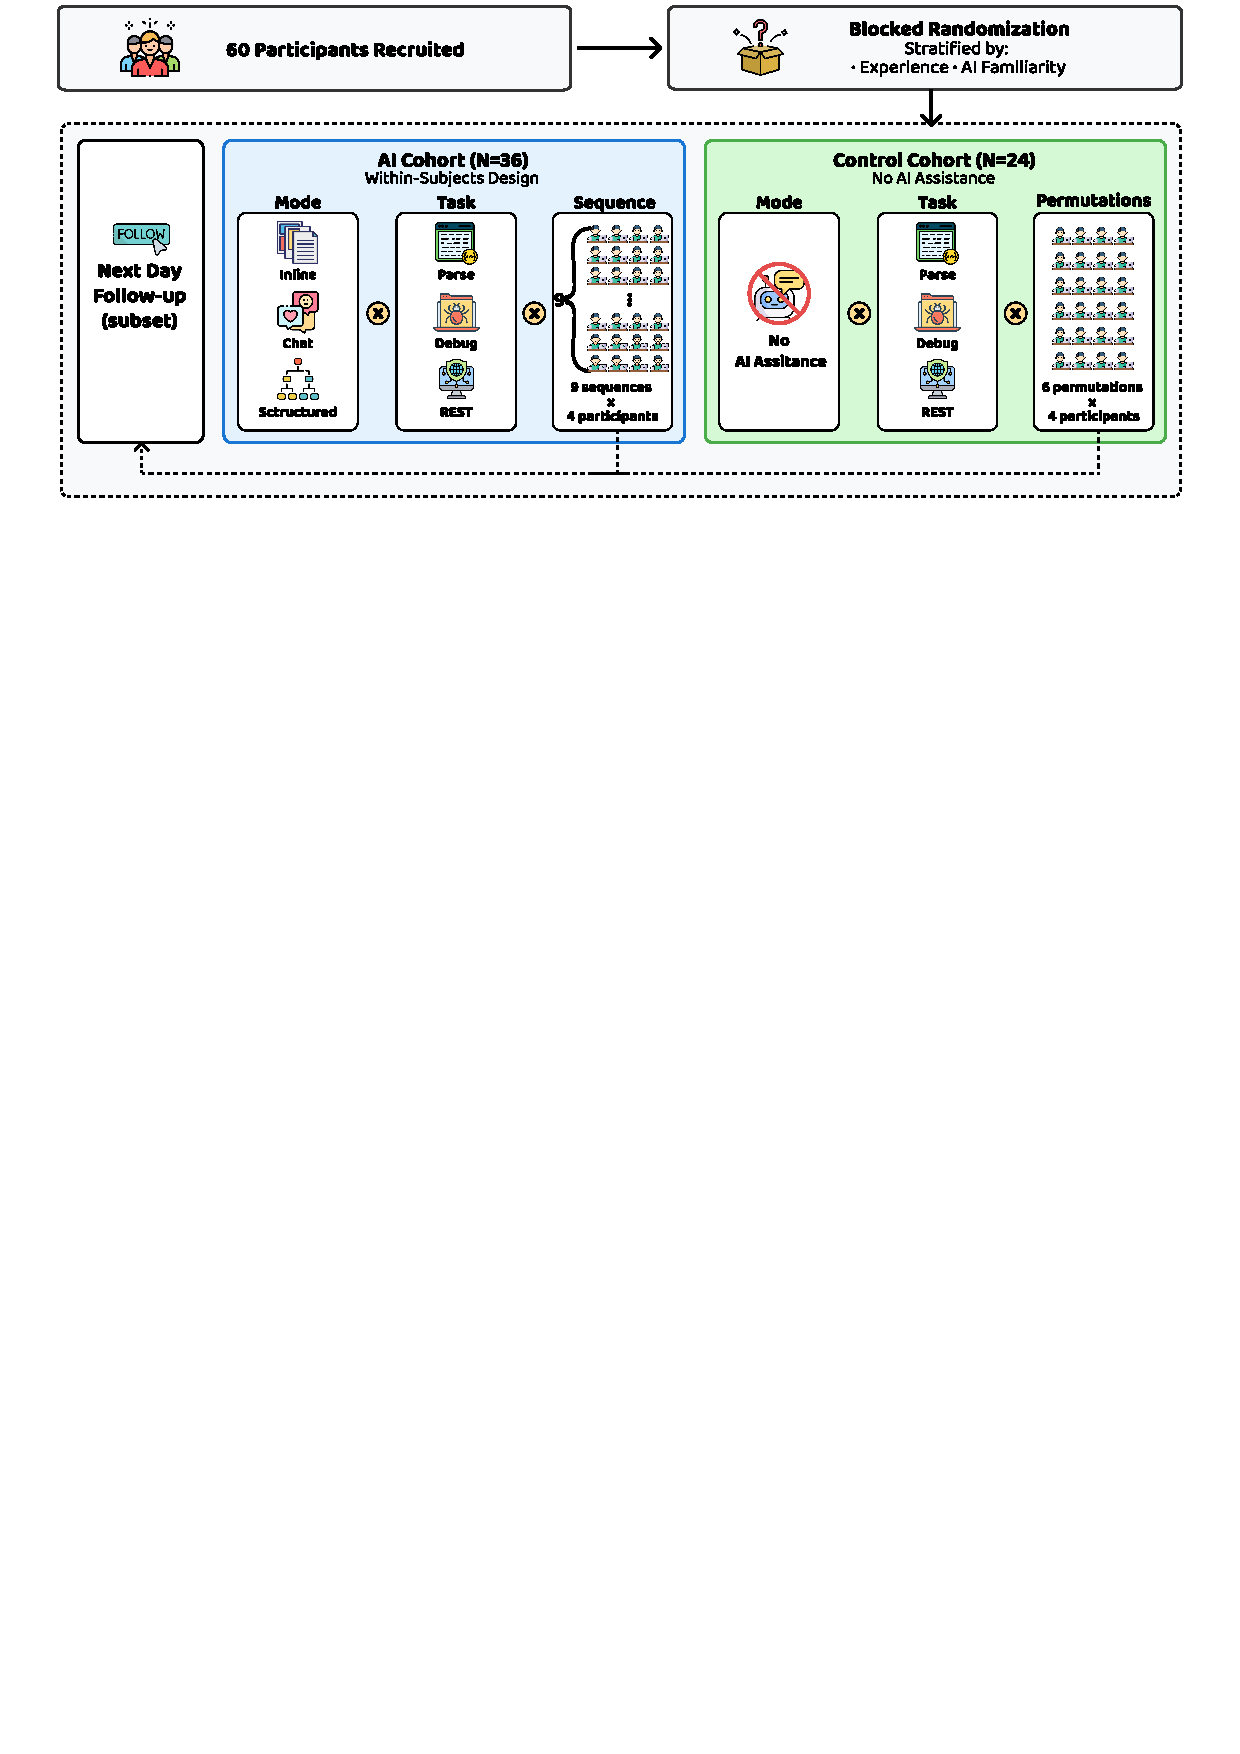
\includegraphics[width=0.99\linewidth]{figures/design.pdf}
  \caption{Study flow, counterbalancing, and measurement timeline. $N{=}60$ randomized to AI ($n{=}36$; within‑subjects comparison of Inline, Chat, Structured across 9 balanced Task$\times$Mode sequences) or Control ($n{=}24$; no‑AI; balanced task orders). Each task block: pre‑task KSS/SSSQ, coding with unified IDE/build logging (events feed the verification‑load composite), post‑task RAW--TLX/KSS/SSSQ; 40\,min cap; 15–20\,min breaks; optional next‑day follow‑up. Only the UI differs; the backend and test oracles are the same. Backend parity: \ModelName\ (\ModelProvider), fixed decoding, no tools/web, state reset.}
  \label{fig:study-flow}
\end{figure*}

\subsection{Participants}
\label{sec:participants}

We recruited $N=60$ participants comprising professional software engineers and advanced computer science students via departmental mailing lists, professional forums, and local developer communities. Inclusion criteria required: (i)~$\geq 2$ years of programming experience, (ii)~proficiency in Python (self-rated $\geq$ intermediate), and (iii)~familiarity with at least one AI-based coding assistant (e.g., ChatGPT, GitHub Copilot, Cursor). Respondents failing to meet criteria were thanked and excluded.

\begin{table}[t]
  \centering
  \caption{Experience bin rubric used for stratification and moderator analysis. Self-efficacy and AI familiarity were measured on 5-point Likert scales (1=low, 5=high).}
  \label{tab:experience-bins}
  \resizebox{\linewidth}{!}{%
  \begin{tabular}{p{0.18\linewidth}p{0.23\linewidth}p{0.24\linewidth}p{0.27\linewidth}}
    \toprule
    \textbf{Bin} & \textbf{Years coding} & \textbf{Self-efficacy} & \textbf{AI familiarity (per-tool)} \\
    \midrule
    Novice & 2--3 & 2--3 & 1--2 (rarely/never) \\
    Intermediate & 3--6 & 3--4 & 2--4 (monthly/weekly) \\
    Experienced & $\geq$6 & 4--5 & 3--5 (weekly/daily) \\
    \bottomrule
  \end{tabular}
  }
\end{table}

Participants were assigned to (a) an AI cohort ($n=36$) or (b) a no-AI control cohort ($n=24$) via blocked randomization stratified by experience bin (Table~\ref{tab:experience-bins}) and per-tool AI familiarity (weekly/daily vs.\ monthly/rarely). This procedure yielded baseline equivalence across cohorts on age, years coding, baseline KSS/SSSQ, and AI familiarity (Section~\ref{sec:descriptives}). To make experience operational and reproducible, we used an explicit binning rubric combining years of programming, self-efficacy ratings, and AI-tool familiarity (Table~\ref{tab:experience-bins}). Per-tool familiarity was captured via frequency-of-use items (Daily/Weekly/Monthly/Rarely/Never) and prior task types performed with each tool (e.g., code generation, debugging, test authoring). We collected age, gender, education, primary languages, and domain specialization (e.g., backend, data, web). We also recorded prior exposure to CSV/JSON parsing, auth/debugging, and REST/batch-processing to control for task-specific familiarity.

\paragraph{Power and sample size.}
We targeted sensitivity to small\hyp{}to\hyp{}medium within-subjects mode effects while preserving a concurrent no-AI trajectory. A preregistered simulation using pilot intraclass correlations indicated $\approx 80\%$ power to detect small-to-medium main effects of \texttt{Mode} on RAW--TLX and log-time within the AI cohort and medium effects for AI vs.\ Control comparisons at $\alpha{=}0.05$ (Holm within contrast families). Details appear in Appendix~\ref{app:power}.
\subsection{Tasks \& Materials}
\label{sec:tasks}

We selected three realistic programming tasks (Table~\ref{tab:task-overview}) in Python to reflect common professional activities while controlling for language-specific confounds. Each task included starter code, unit tests, and a succinct brief describing functional and non-functional requirements. All code and tests will be made available in anonymiz-ed supplemental materials. Tasks A-C cover common professional activities (data parsing, security-relevant debugging, networked batch I/O) with controlled oracles and bounded scope, enabling comparable completion in a single session while eliciting distinct sources of intrinsic complexity (branching, state/clock edge cases, I/O/backoff).

We standardized on Python~3.11 with \texttt{pytest} for unit testing, \texttt{pytest-cov} for coverage, and \texttt{mutmut} for mutation testing. For the REST task we used \texttt{httpx} with a deterministic mock server to control response timing and failure modes. Starter projects included a minimal \texttt{pyproject.toml} and \texttt{requirements.txt}. Each brief specified: (i)~input/output contracts (types and shapes), (ii)~constraints (e.g., no network I/O for Task~A, constant-time token checks for Task~B, bounded concurrency for Task~C), (iii)~interface signatures to implement, and (iv)~acceptance criteria expressed as unit tests. Participants were instructed to ``make tests pass'' and keep changes focused; large refactors were discouraged unless necessary for correctness.

\begin{table}[t]
  \centering
  \caption{Task overview, inputs/outputs, and adequacy of test suites. Static metrics were computed on starter code plus scaffolding; test adequacy summaries are computed on the final reference implementations.}
  \label{tab:task-overview}
  \resizebox{\linewidth}{!}{%
  \begin{tabular}{p{0.1\linewidth}p{0.3\linewidth}p{0.18\linewidth}p{0.12\linewidth}p{0.12\linewidth}p{0.1\linewidth}}
    \toprule
    \textbf{Task} & \textbf{Brief} & \textbf{I/O and APIs} & \textbf{Static metrics} & \textbf{Coverage} & \textbf{Mutation} \\
    \midrule
    \textbf{A: Parse} &
    Implement a robust parser that extracts summary statistics (counts, numeric aggregates) from semi-structured CSV/JSON with missing fields and type noise. Enforce schema validation and produce a typed summary object. &
    Files: CSV/JSON; Output: Python dataclass; No external APIs. &
    LOC $\approx$ 200; median cyclomatic~$\tilde{v} \in [3,5]$; fan-in/out low. &
    Line $\geq 80\%$; Branch $\geq 75\%$ (pytest-cov). &
    Mutation $\geq 60\%$ (mutmut). \\
    \midrule
    \textbf{B: Debug Auth} &
    Diagnose and fix logic errors in a minimal authentication module (password hashing, token issuance, expiry). Improve tests to cover edge cases (clock skew, invalid tokens). &
    In-memory store; \texttt{hashlib}/\texttt{\allowbreak{}secrets}; No network. &
    LOC $\approx$ 260; median cyclomatic~$\tilde{v} \in [4,6]$; moderate branching. &
    Line $\geq 80\%$; Branch $\geq 75\%$. &
    Mutation $\geq 60\%$. \\
    \midrule
    \textbf{C: Batch REST} &
    Extend a REST client to perform batched GET requests with rate limiting, exponential backoff, partial failure handling, and JSON aggregation; log and return per-item status. &
    HTTP via \texttt{httpx}; JSON I/O; Local log. &
    LOC $\approx$ 300; median cyclomatic~$\tilde{v} \in [5,7]$; I/O branching. &
    Line $\geq 80\%$; Branch $\geq 75\%$. &
    Mutation $\geq 60\%$. \\
    \bottomrule
  \end{tabular}
  }
\end{table}

To triangulate task difficulty and avoid advantaging any mode:
\begin{itemize}[leftmargin=1.2em]
  \item \textbf{Expert ratings.} Two senior engineers independently rated perceived complexity (1--5) along structure, branching, and integration dimensions. Inter-rater agreement was substantial ($\kappa \geq 0.70$); disagreements were resolved by discussion.
  \item \textbf{Static metrics.} We computed LOC, cyclomatic complexity (per function and median), and dependency fan-in/out for the starter code. Tasks were targeted to low-to-moderate (A), moderate (B), and moderate-to-high (C) bands without extreme outliers.
  \item \textbf{Pilot equivalence.} A 6-person pilot verified that tasks fell within the intended 20--35 minute window for proficient developers and produced comparable perceived difficulty (no significant differences at $\alpha=0.05$ on a Raw-TLX composite). Briefs and tests were refined to remove ambiguity uncovered in the pilot.
\end{itemize}
For primary models we use \texttt{PreTaskComplexity}, defined as the task-level median cyclomatic complexity computed on the starter code (per task), scaled to $z$ across all observations; this avoids post-treatment bias inherent to per-observation edits. Correctness was operationalized as the number of passing unit tests out of a predefined suite per task (10--12 tests including edge cases). We report line and branch coverage thresholds and mutation scores on the reference implementations (Table~\ref{tab:task-overview}); participant solutions were run against the same suites. Mutation analysis (``kill rate'') served as a sanity check that tests were sensitive to common faults. For Task~C, the mock server produced deterministic error sequences to ensure reproducible backoff behavior.

In addition to task-level static metrics, we computed a per\hyp{}observation complexity score as the median cyclomatic complexity of functions modified by the participant in that task (weighted by lines changed). This continuous metric (z-scored across all observations) is used as \texttt{Complexity} in LMMs; task identity remains in the model to capture non-metric differences. Because the set of functions modified may itself be influenced by \texttt{Mode}, per-observation complexity is treated as an exploratory moderator in RQ3 rather than a covariate in primary RQ1 models to avoid post-treatment bias. Primary models adjust for pre-task complexity using task-level starter-code metrics. While Task~B invites participants to add or refine visible tests as part of the debugging activity, correctness for analysis used a hidden, immutable evaluation suite that was never exposed in the IDE. Participant-authored tests did not affect scoring. To prevent memorization and to diversify starting points, each task had two minor starter variants differing in non-functional details (e.g., identifier names, small refactorings); we denote this as \texttt{TaskVersion} and include it as a random effect in all models.

\subsubsection*{Counterbalancing and Assignment}
\label{sec:counterbalance}

To avoid confounding Task with Mode, we balanced all $3\times3=9$ Task$\times$Mode pairings. We constructed three perfect matchings between Tasks \{A,B,C\} and Modes \{Inline, Chat, Structured\} and rotated task order to balance position (Index 1--3). Table~\ref{tab:pairing-schedule} lists the nine sequence templates; each was instantiated four times (36 AI participants), so each Task$\times$Mode pairing occurred exactly 12 times overall (and 4 times at each Index). Control participants followed balanced task orders with AI disabled. Assignment to sequence templates was randomized with stratification by experience and AI familiarity and was checked with Fisher's exact tests (no associations; see Section~\ref{sec:descriptives}).

\paragraph{Allocation details.}
Sequence templates (Table~\ref{tab:pairing-schedule}) were generated before recruitment and assigned via blocked randomization stratified by \texttt{ExperienceBin} and AI familiarity. Allocation was concealed until session scheduling. Balance checks (Fisher's exact tests) found no association between sequence and experience/familiarity (Section~\ref{sec:descriptives}).

\begin{table}[t]
  \centering
  \caption{Decoupled Task$\times$Mode schedule (AI cohort). Each row shows the (Task, Mode) pair at Index 1, 2, 3. Across the 9 sequences, all 9 Task$\times$Mode pairings are equally represented.}
  \label{tab:pairing-schedule}
  \small
  \begin{tabular}{c c c c}
    \toprule
    \textbf{Seq.} & \textbf{Index 1} & \textbf{Index 2} & \textbf{Index 3} \\
    \midrule
    S1 & (A, Inline) & (B, Chat) & (C, Structured) \\
    S2 & (B, Chat) & (C, Structured) & (A, Inline) \\
    S3 & (C, Structured) & (A, Inline) & (B, Chat) \\
    S4 & (A, Chat) & (B, Structured) & (C, Inline) \\
    S5 & (B, Structured) & (C, Inline) & (A, Chat) \\
    S6 & (C, Inline) & (A, Chat) & (B, Structured) \\
    S7 & (A, Structured) & (B, Inline) & (C, Chat) \\
    S8 & (B, Inline) & (C, Chat) & (A, Structured) \\
    S9 & (C, Chat) & (A, Structured) & (B, Inline) \\
    \bottomrule
  \end{tabular}
\end{table}



\subsection{Interaction Modes}
\label{sec:conditions}

We operationalized three AI interaction modes that are commonly available in professional development environments and controlled the underlying model backend so that differences are attributable to interaction style rather than model capability. Figure~\ref{fig:mode-screens} illustrates the three interfaces; only the UI differed, the LLM backend was identical.


\paragraph{Inline Suggestions (IDE completions).}
Participants used an IDE with inline code completions enabled (e.g., GitHub Copilot–style). Suggestions appeared as ghost text during typing or on demand via a shortcut. Participants could accept, partially accept, or reject suggestions. We instrumented the IDE to log suggestion events (\texttt{offered}, \texttt{accepted}, \texttt{edited-after-accept}, \texttt{rejected}) with timestamps and cursor locations.

\paragraph{Chat-based Interaction (prompt/response).}
Participants interacted with the same LLM backend through a dedicated chat panel (dockable in the IDE). They posed natural-language prompts (e.g., “Explain why these tests fail,” “Generate a batch request loop with retries”), received responses, and could copy/paste code into the editor. We logged prompt turns, response lengths, code-block extractions, and paste events.

\paragraph{Structured Prompts (form schema).}
Participants completed a structured form that constrained the request (schema below): function signature, pre/post-conditions, constraints (e.g., complexity, I/O), error handling, and test hints (edge cases). Submissions triggered LLM code generation and a one-paragraph rationale. We logged field values and generation events.

\begin{quote}
\small
\textbf{Structured prompt schema (excerpt)}\\
\texttt{language}, \texttt{function\_signature}, \texttt{preconditions[]}, \\ \texttt{postconditions[]}, \texttt{constraints[]}, \texttt{error\_handling[]}, \\ \texttt{test\_hints[]}, \texttt{style\_guidelines[]}, \texttt{explanation\_required: bool}
\end{quote}

\noindent\textbf{Permitted affordances per mode.}
Inline: participants could accept full or partial suggestions and immediately edit accepted code. 
Chat: participants could request explanations or code, copy/paste code blocks, and ask follow-ups; no external tools were available.
Structured: participants completed required fields (signature, pre-/post-conditions, constraints, error handling); the form produced code plus a brief rationale.

\noindent\textbf{Unified logging hooks.}
Representative UI snapshots of the three modes appear in Appendix Figure~\ref{fig:mode-screens}.

\noindent\textbf{Unified logging hooks.}
All modes wrote into the same event schema (Appendix Table~\ref{tab:event-log}); Inline logged offer/accept/reject/edit; Chat logged prompt/response turns and paste events; Structured logged field values and generation events. Build/test outcomes were captured uniformly across modes.

\subsubsection*{AI Backend and Configuration}
\label{sec:backend}

\noindent\textbf{Backend parity.}
All modes called the same LLM backend (\ModelName, \ModelProvider, version \ModelVersion) with identical decoding (fixed temperature/top-$p$, max tokens), no tool or web access, and state reset between tasks. Inline suggestions were gated to syntactically stable points; Chat used a fixed system prompt; Structured serialized fields into a canonical prompt template. Full parameters and prompt templates are provided in Appendix~\ref{app:backend}.

\subsection{Measures}
\label{sec:measures}

The main text focuses on why each measure is used, what it reveals for our research questions (RQs), and how to interpret; full instruments, scoring, reliability, event-log fields, and construction details (including PCA checks) appear in Appendix~\ref{app:instruments} and Appendix~\ref{app:analysis-details}.

\paragraph{Workload (RAW NASA--TLX \cite{hart2006nasa}).}
We measured perceived workload with the post-task RAW NASA--TLX, a 0--100 composite averaging Mental Demand, Temporal Demand, Effort, and Frustration. This captures perceived burden beyond speed and correctness and is sensitive to interface-induced \emph{extraneous} load (RQ1). Lower scores indicate lower workload; differences of roughly 5--10 points are typically noticeable. As a subjective, single-task measure, it is interpreted alongside repeated-use KSS/SSSQ and behavioral traces.

\paragraph{Completion time (minutes).}
Completion time is defined as minutes from the first keystroke to the first fully passing test suite. It serves as a direct productivity proxy under identical oracles (RQ1); lower values indicate faster completion. We model time on the log scale to handle skew and report back-transformed means and time ratios (e.g., a ratio of $0.78$ corresponds to 22\% faster), with right-censoring at 40\,min addressed via log models and AFT sensitivity checks.

\paragraph{Correctness.}
Correctness is the number of unit tests passed out of a task-specific suite ($N{=}10$--12), providing a comparable outcome-quality indicator across modes (RQ1). Higher values indicate better solutions, and between-mode differences are summarized using odds ratios from GLMMs. Because test suites are proxies for true correctness, mutation and coverage analyses in Appendix~\ref{app:tasks-metrics} support their adequacy.

\paragraph{Fatigue (Karolinska Sleepiness Scale, KSS \cite{kaida2006validation}).}
Fatigue is measured with the Karolinska Sleepiness Scale (1 = alert, 9 = very sleepy) administered pre- and post-task. This tracks cumulative tiredness across repeated tasks where TLX may not (RQ2); lower scores indicate more alertness, and we model both post-task levels and pre–post changes ($\Delta$). As a single-item measure, KSS is interpreted in conjunction with SSSQ and behavioral mediators.

\paragraph{Stress (Short Stress State Questionnaire, SSSQ \cite{helton2015short}).}
Stress is assessed with the Short Stress State Questionnaire, computed as a post-task composite and standardized to $z$-scores. This captures distress and worry beyond effort (RQ2); lower $z$ indicates lower stress. As a self-report measure, SSSQ patterns are triangulated with behavioral traces.

\paragraph{Verification-load composite $V_{\text{core}}$ (mode-agnostic).}
Verification load $V_{\text{core}}$ is the mean $z$-score across five uniformly logged signals: (i) compile/test failures, (ii) time-to-first-compile, (iii) normalized code churn, (iv) cumulative pauses $>$2\,s, and (v) context switches (editor$\leftrightarrow$tests$\leftrightarrow$chat/form). This composite operationalizes the \emph{process cost of checking and repairing} model output across interfaces, aligning with cognitive-load and flow/interruptions theory (RQ2/\\RQ3). Values are unitless within-task $z$-scores, where $0$ is typical and higher values indicate greater verification burden; an equal-weight scheme is used for portability, with PCA-weighted and mode-extended variants ($V_{\text{plus}}$) reported in Appendix~\ref{app:analysis-details}.

\paragraph{Mode-specific signals (secondary).}
We also log mode-specific traces, including inline acceptance/rejection densities and Chat prompt turns/pastes, as diagnostic context for mode differences and sensitivity checks. Calibrated acceptance (neither near-0 nor near-1) is descriptively associated with higher correctness, but these signals are not directly comparable across modes and are therefore excluded from $V_{\text{core}}$.

Reliability (e.g., TLX $\alpha$, SSSQ $\alpha$), logging coverage ($>\!99\%$ for key events), missingness ($<\!2\%$), and imputation checks are summarized in the Results and detailed in Appendix~\ref{app:instruments} and Appendix~\ref{app:analysis-details}.
\subsection{Procedure}
\label{sec:procedure}

Participants reviewed consent, demographics, and expertise/familia-rity items, then completed a 5--7\,min warm-up with IDE, test runner, and (AI cohort) all three interaction modes. For each task, we administered KSS and SSSQ pre and post. Each participant completed three tasks separated by 15--20\,min breaks. The task schedule followed the balanced templates in Table~\ref{tab:pairing-schedule} (AI) or a balanced task order (Control). A 40\,min cap per task was enforced. If no full pass was achieved by the cap, time was right-censored at 40\,min and a completion indicator was recorded; survival (AFT) models serve as robustness checks for time outcomes. 

A subset returned the next day to repeat a matched-complexity task in their assigned condition. We re-administered SSSQ/KSS and logged the same behavioral/performance measures to assess short-term recovery and persistence of preferences. Lab sessions used identical workstations; remote sessions mirrored the setup with a provided container image. All sessions were screen-recorded; only derived action codes (navigation, acceptance/rejection, re-runs, context switches) are released. Personally identifying information never appeared in logs. Appendix Figure~\ref{fig:timeline} summarizes the within‑task measurement timeline and enforced breaks.

\noindent\textbf{Environment parity.}
Lab and remote sessions used the same containerized setup; the \texttt{Environment} factor was included in models and did not alter inferences (Section~\ref{sec:descriptives}).

% -----------------------------------------------------

\subsection{Instrumentation \& Logging Reliability}
\label{sec:logging-reliability}
We synchronized IDE and test-harness clocks via a handshake at task start; median drift was $<\!50$\,ms and corrected during alignment. Event coverage exceeded 99\% for offers/accepts/rejects, prompts, compile/test runs. Missingness was $<\!2\%$ overall and treated as MCAR (Appendix~\ref{app:data-qc}); primary analyses used listwise deletion with multiple imputation as a sensitivity check (robust).

\section{Data Analysis}
\label{sec:analysis}

We map analysis choices directly to the RQs and report effects in units that are easy to read (points, minutes/ratios, odds ratios). Full model syntax, diagnostics, robustness, and equivalence tests appear in Appendix~\ref{app:stats-spec} and \ref{app:analysis-details}.

For \textbf{RQ1}, we compare Inline, Chat, and Structured on workload, time, and correctness using mixed‑effects models that adjust for task, order, and experience. Workload (TLX) and time use linear mixed‑effects models (LMMs) with random intercepts for participants and task variant; time is modeled on the log scale but reported back‑transformed in minutes alongside time ratios. Correctness uses a binomial GLMM (logit link) over tests passed out of $N$. These choices isolate interface effects while accounting for repeated measures and task heterogeneity.

For \textbf{RQ2}, we estimate fatigue (KSS) and stress (SSSQ) slopes across Task Index (1$\rightarrow$3) with LMMs; when supported, we include random slopes for Index by participant to capture individual trajectories. To examine mechanism, we use a two‑equation mediation: Index (or Mode) predicts the verification‑load composite $V_{\text{core}}$, and $V_{\text{core}}$ predicts outcomes while controlling for Index/Mode and covariates. Indirect effects are estimated via Monte‑Carlo simulation with bootstrap sensitivity; we interpret significant indirect paths as \emph{consistent with} a verification‑load mechanism rather than causal proof.

For \textbf{RQ3}, we include interactions with expertise bins and with continuous per‑observation complexity. We then use Johnson\hyp{}Neyman regions to state where, along the complexity continuum, one mode reliably overtakes another. This avoids arbitrary binning and yields actionable thresholds.

Across models we include, unless noted, fixed effects for \texttt{Mode} (or \texttt{Condition:} AI vs Control), \texttt{Task}, \texttt{Task Index} (1–3), \texttt{Experience-\allowbreak{}Bin}, \texttt{AI\_Familiarity}, \texttt{PreTaskComplexity} (task‑level), and \texttt{Envi-\allowbreak{}ronment} (lab/remote), plus random intercepts for \texttt{Participant} and \texttt{TaskVersion}; when convergence and fit support it, we add random slopes for Index. We report estimated marginal means with 95\% CIs, Holm-adjusted $p$‑values within contrast families, and effect sizes in practical units: TLX point differences (negative is better), back‑transformed minutes and time ratios (e.g., $0.78{=}$22\% faster), and odds ratios for correctness ($>$1 favors the named mode). For KSS/SSSQ we report post‑task levels and slopes (lower is better; SSSQ as $z$). Multiplicity is controlled via Holm adjustments; where we claim “no practically important difference,” we use TOST equivalence with preregistered bounds (±5 TLX points, ±5\% time ratio, ±0.5/10 tests). Robustness checks (AFT survival for time to handle right‑censoring, ordinal models for TLX, alternative links for correctness), influence diagnostics, and multiple‑imputation results are in Appendix~\ref{app:analysis-details}. The main analytical limitations are that $V_{\text{core}}$ is observational and Johnson–Neyman regions inherit uncertainty from the fitted interactions; we temper claims accordingly and rely on convergence between subjective, behavioral, and outcome evidence.
% ---------- Concise Ethics & Privacy paragraph ----------
\subsection{Ethics \& Privacy}
\label{sec:ethics}

All procedures were approved by our institutional ethics board. Participants provided written informed consent prior to any study activity (with an additional oral confirmation for remote sessions). We minimized personal data collection and assigned pseudonymous IDs at intake; demographic records and interaction logs were stored separately on encrypted servers with access restricted to the research team. Screen recordings were collected solely for within-team analysis. Prompt and response texts were hashed in logs to reduce risks of sensitive content disclosure, and any incidental identifiers were redacted during data cleaning. Participants were informed of their right to withdraw at any time without penalty. Assistant requests contained only task code and prompts; no external tools or web retrieval were enabled. Prompt and response texts were hashed in logs; no raw conversational content or personal identifiers were stored.


\section{Results}
\label{sec:results}

\subsection{Descriptives \& Checks}
\label{sec:descriptives}

\paragraph{Sample and exposure.}
We analyzed $N=60$ participants (AI $n{=}36$, Control $n{=}24$), producing $180$ task-level observations (AI: $108$; Control: $72$). Experience bins were balanced across cohorts (AI: Novice $=12$, Intermediate $=16$, Experienced $=8$; Control: $8/12/4$). Weekly/daily familiarity was common for ChatGPT ($78\%$) and frequent for Copilot ($62\%$), lower for CodeWhisperer ($18\%$). All participants met the Python~3.11 proficiency criterion; secondary languages included JavaScript/TypeScript ($48\%$) and Java ($35\%$). Table~\ref{tab:profile} summarizes cohort composition and weekly/daily tool familiarity.


\paragraph{Counterbalancing integrity.}
The AI cohort used nine decoupled Task$\times$Mode sequences (Table~\ref{tab:pairing-schedule}), instantiated exactly four times each (4 participants per sequence; 36 total). By construction, all $3{\times}3=9$ Task$\times$Mode cells occurred equally often (12 observations per cell) and each Mode occurred equally often at each Index (1--3). No dropouts occurred. A post-hoc check found no association between sequence template and experience bin (Fisher’s exact $p{=}0.88$). The Control cohort used balanced task orders (six permutations, 4 participants per order); no association with experience bin was detected (Fisher’s exact $p{=}0.90$).
\paragraph{Cohort baseline equivalence.}
AI and Control cohorts were comparable at baseline (Table~\ref{tab:baseline-eq}); all standardized mean differences (SMD) were $<0.20$ in magnitude with 95\% CIs spanning zero.

\begin{table}[t]
  \centering
  \caption{Baseline equivalence (mean$\pm$SD; standardized mean differences, SMD).}
  \label{tab:baseline-eq}
  \small
  \resizebox{\linewidth}{!}{%
  \begin{tabular}{lccc}
    \toprule
    \textbf{Variable} & \textbf{AI} & \textbf{Control} & \textbf{SMD [95\% CI]} \\
    \midrule
    Age (years) & $27.4\pm3.1$ & $27.1\pm3.2$ & $0.06\,[-0.24,\,0.35]$ \\
    Years coding & $5.1\pm2.8$ & $4.9\pm2.6$ & $0.07\,[-0.22,\,0.36]$ \\
    KSS (pre Task~1) & $3.1\pm1.2$ & $3.2\pm1.1$ & $-0.05\,[-0.34,\,0.25]$ \\
    SSSQ (pre Task~1, $z$) & $-0.02\pm0.98$ & $0.03\pm1.01$ & $-0.05\,[-0.35,\,0.25]$ \\
    AI familiarity (wk/dy; proportion) & 0.69 & 0.67 & 0.05\,[-0.25,\,0.35]  \\
    \bottomrule
  \end{tabular}
  }
\end{table}
\paragraph{Task difficulty comparability and complexity checks.}
Static metrics confirmed the intended structural ordering (median cyclomatic: Task~A $3.9$, Task~B $4.8$, Task~C $6.1$). Using the per-observation complexity metric (median cyclomatic of functions modified, weighted by lines changed; z-scored), we observed no imbalance across \texttt{Mode} or \texttt{Index} in the AI cohort (LMM with participant random intercept: \texttt{Mode} $\chi^2(2){=}1.42$, $p{=}0.49$; \texttt{Index} $\chi^2(2){=}0.97$, $p{=}0.62$). In the Control cohort, RAW--TLX composites differed modestly by task (A: $\bar{x}{=}71.2$, B: $75.0$, C: $77.5$), but with \texttt{Index} and experience covariates in a mixed model, the \texttt{Task} main effect was small and not significant ($\chi^2(2){=}3.18$, $p{=}0.20$), indicating comparability sufficient for Mode contrasts.
\paragraph{Instrument reliability, distributions, and censoring.}
Internal consistency was acceptable to good: RAW--TLX composite $\alpha{=}0.86$; SSSQ $\alpha{=}0.81$. KSS showed acceptable test--retest stability across Task~1 baselines ($r{=}0.72$). Completion time was positively skewed and analyzed on the log scale. Right-censoring at the 40\,min cap affected $11/180$ tasks (6.1\%; AI $=7$, Control $=4$; Fisher’s exact $p{=}0.63$); accelerated failure time (AFT) models confirmed the direction and significance of time effects (Section~\ref{sec:rq1}). Missing data were minimal ($<1.7\%$) and listwise deletion yielded the same pattern as multiple imputation (supplement).
\paragraph{Logging coverage.}
Event logs covered $>\!99\%$ of key actions (offers/accepts/rejects, prompts, compile/test runs); post\hyp{}synchronization timestamp drift (IDE vs.\ test harness) averaged $<50$\,ms.

\begin{table}[t]
  \centering
  \caption{Participant profile by cohort and experience; per-tool familiarity is weekly/daily usage.}
  \label{tab:profile}
  \small
  \begin{tabular}{lcccc}
    \toprule
    & \textbf{AI} & \textbf{Control} & \textbf{Total} & \textbf{\%} \\
    \midrule
    Novice & 12 & 8 & 20 & 33.3 \\
    Intermediate & 16 & 12 & 28 & 46.7 \\
    Experienced & 8 & 4 & 12 & 20.0 \\
    \midrule
    ChatGPT (wk/dy) & \multicolumn{4}{c}{78\%} \\
    Copilot (wk/dy) & \multicolumn{4}{c}{62\%} \\
    CodeWhisperer (wk/dy) & \multicolumn{4}{c}{18\%} \\
    \bottomrule
  \end{tabular}
\end{table}


\subsection{RQ1 — Immediate Effects of Interaction Mode on Workload, Time, and Correctness}
\label{sec:rq1}
\begin{figure*}[t]
  \centering
  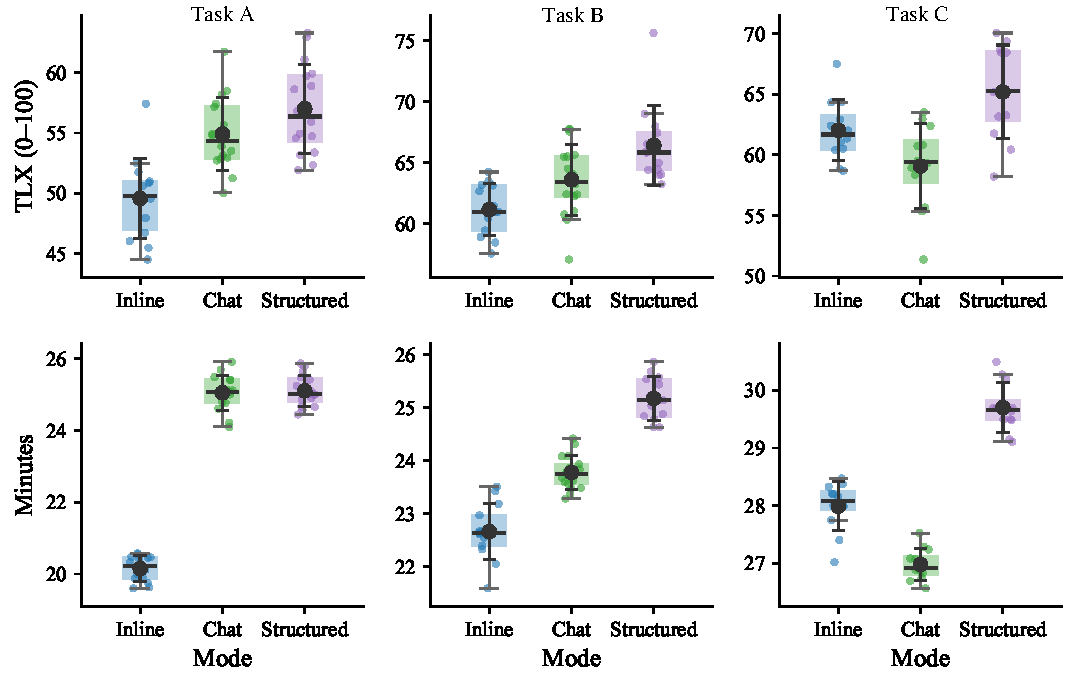
\includegraphics[width=0.9\linewidth]{figures/rq1_tlx_time_combo(1).pdf}
\caption{NASA--TLX workload scores and completion times across tasks and three AI modes. (Top) Inline yields lower workload on low-complexity tasks; differences narrow as complexity increases. (Bottom) Completion times by task complexity. On the highest-complexity task (C), Chat and Inline are comparable (EMMs 27.1 vs.\ 27.8 minutes) and both faster than Structured (29.7 minutes), indicating that Chat's speed does not degrade at high complexity.}
  \label{fig:rq1-tlx-time}
\end{figure*}

\begin{table}[t]
  \centering
  \caption{Estimated marginal means (EMMs) by Mode $\times$ Task for primary outcomes. Time back-transformed to minutes; Correctness shown as tests passed out of 10 (Task A,C) or 12 (Task B) with EMM scaled to /10 for comparability. 95\% CIs in brackets.}
  \label{tab:rq1-emms}
  \small
  \resizebox{\linewidth}{!}{%
  \begin{tabular}{l l c c c}
    \toprule
    \textbf{Task} & \textbf{Mode} & \textbf{TLX (0--100)} & \textbf{Time (min)} & \textbf{Correctness (/10)} \\
    \midrule
    A (low) & Inline     & 49.3 [45.6, 53.0] & 19.9 [18.5, 21.3] & 8.3 [8.0, 8.6] \\
            & Chat       & 56.0 [52.1, 60.0] & 24.5 [22.7, 26.4] & 8.2 [7.9, 8.5] \\
            & Structured & 58.1 [54.3, 61.9] & 25.1 [23.3, 27.0] & 8.3 [8.0, 8.6] \\
    \midrule
    B (mid) & Inline     & 55.4 [51.7, 59.1] & 22.5 [21.0, 24.1] & 7.2 [6.9, 7.5] \\
            & Chat       & 58.1 [54.4, 61.8] & 23.9 [22.2, 25.7] & 7.3 [7.0, 7.6] \\
            & Structured & 60.9 [57.2, 64.6] & 25.0 [23.2, 26.9] & 7.6 [7.3, 7.9] \\
    \midrule
    C (high)& Inline     & 60.9 [57.3, 64.6] & 27.8 [26.0, 29.8] & 7.3 [6.9, 7.7] \\
            & Chat       & 59.7 [56.1, 63.2] & 27.1 [25.4, 28.9] & 8.0 [7.6, 8.5] \\
            & Structured & 66.0 [62.5, 69.4] & 29.7 [27.9, 31.8] & 7.1 [6.7, 7.5] \\
    \bottomrule
  \end{tabular}
  }
\end{table}
We compared the three AI modes within the AI cohort and contrasted AI (pooled) against the no-AI Control. Models (Section~\ref{sec:analysis}) included fixed effects for \texttt{Mode}, \texttt{Task}, \texttt{Index}, \texttt{ExperienceBin}, \texttt{AI\_Familiarity}, \texttt{PreTaskComplexity}, and \texttt{Environment} (lab/remote), with random intercepts for participants and task version and random slopes for \texttt{Index} where convergent. Table~\ref{tab:rq1-emms} reports Mode$\times$Task estimated marginal means (EMMs) for TLX, time, and correctness.

\paragraph{Workload (RAW--TLX).}
AI reduced post-task workload relative to Control (EMM difference ${-}18.2$ TLX points on a 0--100 scale, 95\%\,CI $[{-}22.3, {-}14.0]$, $p<0.001$). Within AI, \texttt{Mode} and \texttt{Mode$\times$Task} were significant (Type~III LRTs: $\chi^2(2){=}30.7$, $p<0.001$; $\chi^2(4){=}12.9$, $p{=}0.011$). On low-complexity Task~A, Inline produced the lowest TLX (EMM $=49.3$, CI $[45.6, 53.0]$), outperforming Chat (56.0 $[52.1, 60.0]$, $\Delta{=}{-}6.7$ TLX points, $p{=}0.006$ Holm-adjusted) and Structured (58.1 $[54.3, 61.9]$, $\Delta{=}{-}8.8$ TLX points, $p<0.001$). On moderate Task~B, Inline retained a TLX advantage over Structured ($\Delta{=}{-}5.5$ TLX points, $p{=}0.024$), while Inline vs.\ Chat was smaller and not significant after correction ($\Delta{=}{-}3.1$ TLX points, $p{=}0.14$). On higher-complexity Task~C, Chat and Inline were statistically indistinguishable (Chat 59.7 $[56.1, 63.2]$ vs.\ Inline 60.9 $[57.3, 64.6]$, $p{=}0.48$), both below Structured (66.0 $[62.5, 69.4]$; Chat--Structured $\Delta{=}{-}6.3$ TLX points, $p{=}0.008$). \texttt{Environment} was not a significant predictor ($p{=}0.61$). Figure~\ref{fig:rq1-tlx-time} visualizes TLX patterns by task and mode.

\paragraph{Completion time.}
Completion time (log-minutes) showed a strong \texttt{Mode} main effect ($\chi^2(2){=}27.6$, $p<0.001$) and \texttt{Mode$\times$Task} interaction ($\chi^2(4){=}11.1$, $p{=}0.025$). Back-transformed EMMs (minutes) indicated Inline was fastest on Task~A (19.9\,min, CI $[18.5, 21.3]$) compared to Chat (24.5 $[22.7, 26.4]$, $p<0.001$) and Structured (25.1 $[23.3, 27.0]$, $p<0.001$). On Task~B, Inline remained faster (22.5\,min) than Structured (25.0\,min, $p{=}0.014$); Inline vs.\ Chat narrowed (23.9\,min; $p{=}0.08$). On Task~C, Chat (27.1\,min) and Inline (27.8\,min) were comparable ($p{=}0.56$) and both faster than Structured (29.7\,min, $p{=}0.021$). Pooled across tasks, AI was 22\% faster than Control (time ratio $=0.78$, 95\%\,CI $[0.74, 0.83]$, $p<0.001$; AI: 25.0\,min vs.\ Control: 32.1\,min). AFT survival models (log-normal) yielded consistent hazard ratios (Inline vs.\ Structured HR$=1.32$, 95\%\,CI $[1.12, 1.56]$; Chat vs.\ Structured HR$=1.17$ $[1.00, 1.37]$), confirming robustness to right-censoring at 40\,min. Figure~\ref{fig:rq1-tlx-time} (bottom) shows the corresponding completion times.
\begin{figure*}[t]
  \centering
  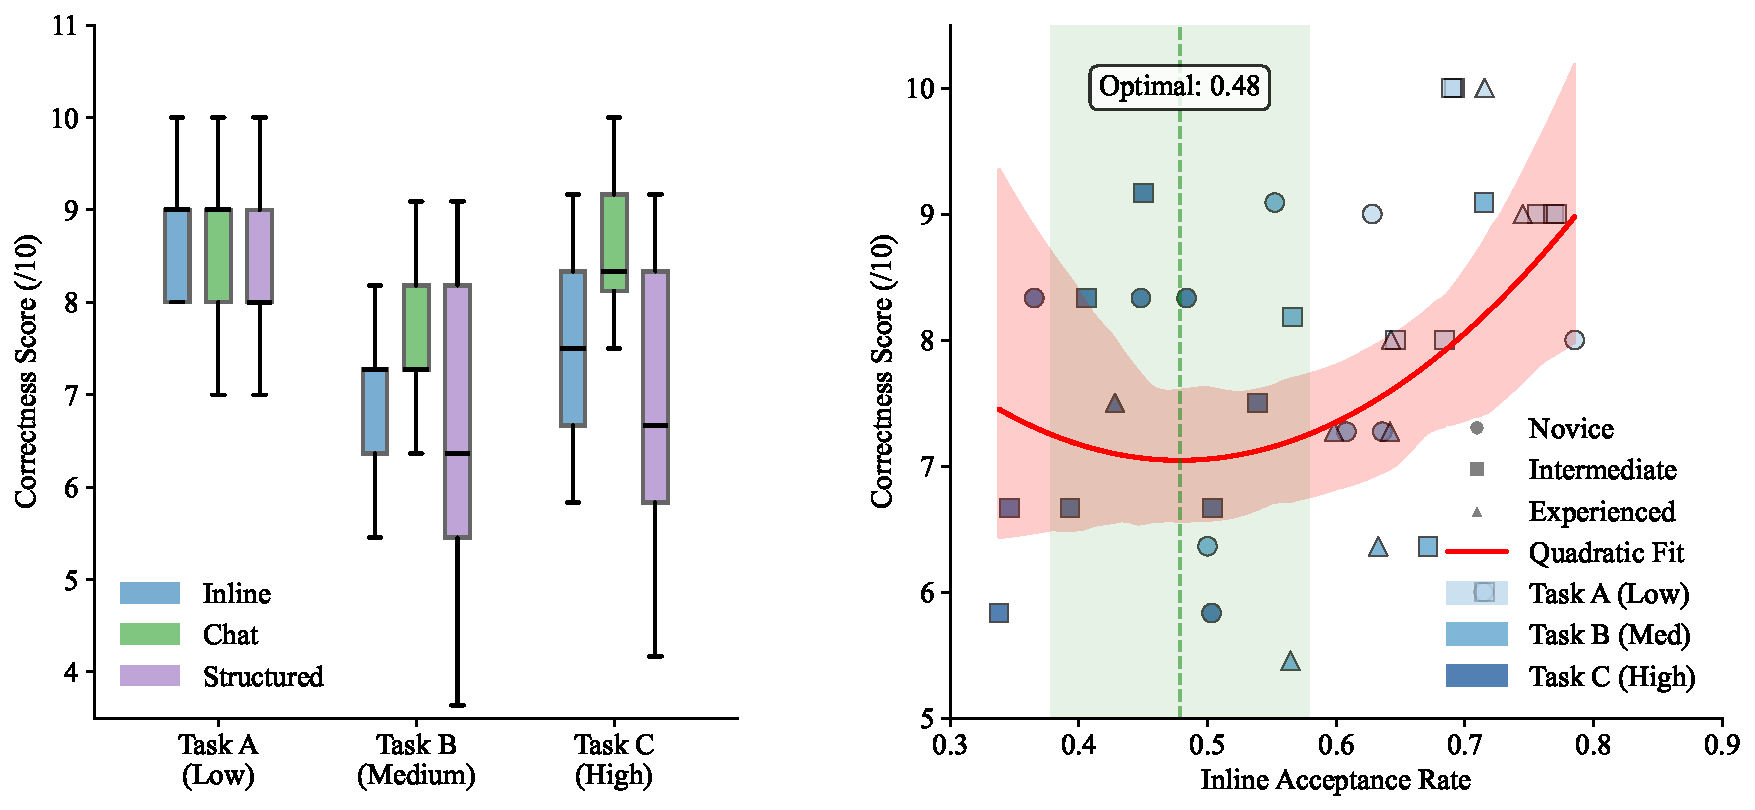
\includegraphics[width=0.9\linewidth]{figures/figure2_correctness.pdf}
  \caption{Code Correctness and AI Suggestion Acceptance Patterns. (Left) Box plots of correctness scores by mode and complexity. Chat excelled at high complexity, while Inline performed best at low complexity. (Right) Quadratic relationship between Inline acceptance rate and correctness, with optimal performance at $\approx 50\%$ acceptance ($\hat{p}=0.48$, 95\% CI quadratic fit shown). Points sized by verification load.}

  \label{fig:rq1-correctness}
\end{figure*}
\paragraph{Correctness.}
Figure~\ref{fig:rq1-correctness} contrasts correctness by mode and complexity. A binomial GLMM (\# passed out of task-specific $N$) revealed \texttt{Mode$\times$Task} as a significant predictor of correctness ($\chi^2(4){=}12.1$, $p{=}0.016$). On Task~C (higher complexity), Chat achieved the highest EMM (8.0/10, CI $[7.6, 8.5]$), exceeding Inline (7.3 $[6.9, 7.7]$, $p{=}0.009$) and Structured (7.1 $[6.7, 7.5]$, $p{=}0.005$). On Task~B (moderate), Structured modestly outperformed Inline (7.6 vs.\ 7.2; $p{=}0.041$) and was comparable to Chat (7.3; $p{=}0.12$). On Task~A (low), all modes clustered near 8.3/10 with no reliable differences after Holm correction ($p>0.10$). Across tasks, AI (pooled) exceeded Control (AI EMM $=$ 7.6/10, Control $=$ 6.2/10; odds ratio $=$ 1.71, CI $[1.37, 2.13]$, $p<0.001$).
\paragraph{Trust and usability}
UMUX-Lite usability was high across modes (EMMs 79--82/100) with no reliable differences after Holm correction. Trust in automation showed the same qualitative pattern and did not alter the main Mode effects when added as a covariate.

\paragraph{Supporting behavioral indicators.}
Inline exhibited higher suggestion acceptance on Task~A (mean $0.60$, SD $0.18$) and shorter cumulative pauses (median $=2.9$\,min) than Chat (pauses $=3.7$\,min) and Structured ($=4.0$\,min). On Task~C, Chat involved more prompt turns (median $=4$) yet fewer compile--fail loops prior to a passing run (median $=1$) than Inline (median $=2$) and Structured (median $=3$), consistent with iterative clarification mitigating error cascades. Figure~\ref{fig:rq1-correctness} (right) shows the Inline acceptance--correctness curve; a quadratic term for acceptance rate significantly predicted correctness (Wald $p{=}0.005$), with an estimated optimum at $\hat{p}{\approx}0.48$ (95\% CI $[0.44, 0.53]$). We treat this "sweet spot" as exploratory rather than prescriptive; calibrated use outperforms both blind acceptance and near-total rejection.

\textbf{AI vs.\ Control.} AI lowered workload (\(-18.2\) RAW--TLX points), reduced time (\(\times 0.78\)), and improved correctness (OR \(=1.71\)). \textbf{Within AI.} Inline is fastest and lowest-load on low complexity; as complexity rises, Chat yields higher correctness without a time penalty; Structured offers modest advantages at mid complexity, especially for novices. 
\textbf{Behavioral alignment.} Inline shows higher acceptance and fewer pauses on simple work; Chat shows more prompt turns but fewer compile–fail loops on complex work.


\subsection{RQ2 — Repeated-Use Trajectories (Stress \& Fatigue)}
\label{sec:rq2}
We modeled post-task fatigue (KSS) and stress (SSSQ) as a function of \texttt{Condition} (AI vs.\ Control), \texttt{Index} (task position: 1--3), \texttt{Task}, \texttt{ExperienceBin}, continuous \texttt{Complexity} (per-observation $z$), and \texttt{Environment} (lab/remote), with random intercepts for participants and task version and random slopes for \texttt{Index} where convergent (Section~\ref{sec:analysis}). Figure~\ref{fig:rq2-trajectories} shows Condition$\times$Index trajectories with 95\% CIs.

\paragraph{Fatigue (KSS).}
Fatigue increased across the three tasks in both cohorts (\texttt{Index} main effect: $\chi^2(1){=}22.1$, $p<0.001$). The \texttt{Condition$\times$\allowbreak{}Index} interaction was significant ($\chi^2(1){=}4.2$, $p{=}0.041$): adjusted means rose by $\Delta{=}{+}0.70$ KSS points from Task~1 to Task~3 for AI, versus $\Delta{=}{+}0.48$ for Control (Table~\ref{tab:rq2-slopes}). Allowing random slopes for \texttt{Index} improved fit (AIC $\downarrow$) without changing fixed-effect inferences.

\paragraph{Stress (SSSQ).}
Post-task SSSQ also increased with \texttt{Index} ($\chi^2(1){=} \allowbreak{} 8.7$, $p{=}0.003$). The \texttt{Condition$\times$Index} term was positive but not significant at conventional levels after multiplicity control ($p{=}0.110$), with a numerically steeper slope in AI (post-task SSSQ $z$-score $\Delta{=}{+}0.17$) than Control ($+0.07$).

\paragraph{Per-mode slopes within AI.}
Within AI, \texttt{Mode$\times$Index} was significant for KSS ($\chi^2(2){=}6.8$, $p{=}0.033$): Inline exhibited a steeper fatigue increase (EMM $\Delta{=}{+}1.18$) than Chat ($+0.92$, $\Delta{=}0.26$, $p{=}0.048$) with Structured in-between ($+1.05$, Inline--Structured $p{=}0.19$). SSSQ showed the same ordering but did not reach significance after adjustment. See Appendix Table~\ref{tab:per-mode-slopes} for the full numerical summaries.

\begin{table}[h]
  \centering
  \caption{Condition$\times$Index trajectory estimates for fatigue (KSS) and stress (SSSQ). $\Delta$ is Task~3 minus Task~1 adjusted mean.}
  \label{tab:rq2-slopes}
  \small
  \begin{tabular}{lcc}
    \toprule
    & \textbf{KSS $\Delta$ [95\% CI]} & \textbf{SSSQ $\Delta$ (z) [95\% CI]} \\
    \midrule
    AI      & +0.70\ [0.48, 0.92] & +0.17\ [0.06, 0.28] \\
    Control & +0.48\ [0.28, 0.68] & +0.07\ [\!-0.01, 0.15] \\
    \midrule
    $p$ (Cond$\times$Index) & 0.041 (KSS) & 0.110 (SSSQ) \\
    \bottomrule
  \end{tabular}
\end{table}

\paragraph{Mediation by verification-load ($V_{\text{core}}$; AI cohort).}
Using the mode-agnostic composite $V_{\text{core}}$, a-paths (\texttt{Index}$\to V_{\text{core}}$) were positive ($\hat{a}{=}0.19$, SE$=0.06$, $p{=}0.002$) and b-paths ($V_{\text{core}}\to Y$) were positive for both outcomes (KSS: $\hat{b}{=}0.78$, SE$=0.22$, $p<0.001$; SSSQ: $\hat{b}{=}0.43$, SE$=0.16$, $p{=}0.007$). Monte Carlo estimates yielded indirect effects of $ab_{\text{KSS}}=0.15$ [0.06, 0.27] and $ab_{\text{SSSQ}}=0.08$ [0.03, 0.16], corresponding to approximately 26\% and 24\% of the total \texttt{Index} effect, respectively. Including $V_{\text{core}}$ improved model fit (KSS: $\Delta$AIC $={-}10.9$) and raised marginal $R^2$ (0.18 $\to$ 0.26). As a sensitivity check, an extended composite $V_{\text{plus}}$ that adds mode-specific signals (Inline acceptance/rejection, Chat prompt turns) produced slightly larger indirect effects (KSS $ab{=}0.19$ [0.08, 0.32]; SSSQ $ab{=}0.11$ [0.04, 0.20]) with unchanged conclusions. Table~\ref{tab:rq2-mediation} summarizes the $a$/$b$ paths and Monte Carlo indirect effects. We interpret these indirect effects as consistent with partial mediation; the design does not establish causal identification.


\begin{table}[t]
  \centering
  \caption{Mediation of Index $\rightarrow$ outcomes via $V_{\text{core}}$ in AI cohort. Indirect effect ($ab$) from 10{,}000-draw Monte Carlo with cluster-robust SEs.}
  \label{tab:rq2-mediation}
  \small
  \begin{tabular}{lccc}
    \toprule
    \textbf{Outcome} & \textbf{$a$ (Index$\to V_{\text{core}}$)} & \textbf{$b$ ($V_{\text{core}}\to Y$)} & \textbf{$ab$ [95\% CI]} \\
    \midrule
    KSS    & 0.19\ (0.06)$^{**}$ & 0.78\ (0.22)$^{***}$ & 0.15\ [0.06, 0.27] \\
    SSSQ z & 0.19\ (0.06)$^{**}$ & 0.43\ (0.16)$^{**}$  & 0.08\ [0.03, 0.16] \\
    \midrule
    \multicolumn{4}{l}{\footnotesize Notes: entries show estimate (SE); $^{**}p<.01$, $^{***}p<.001$.} \\
    \bottomrule
  \end{tabular}
\end{table}


\begin{figure*}[t]
  \centering
  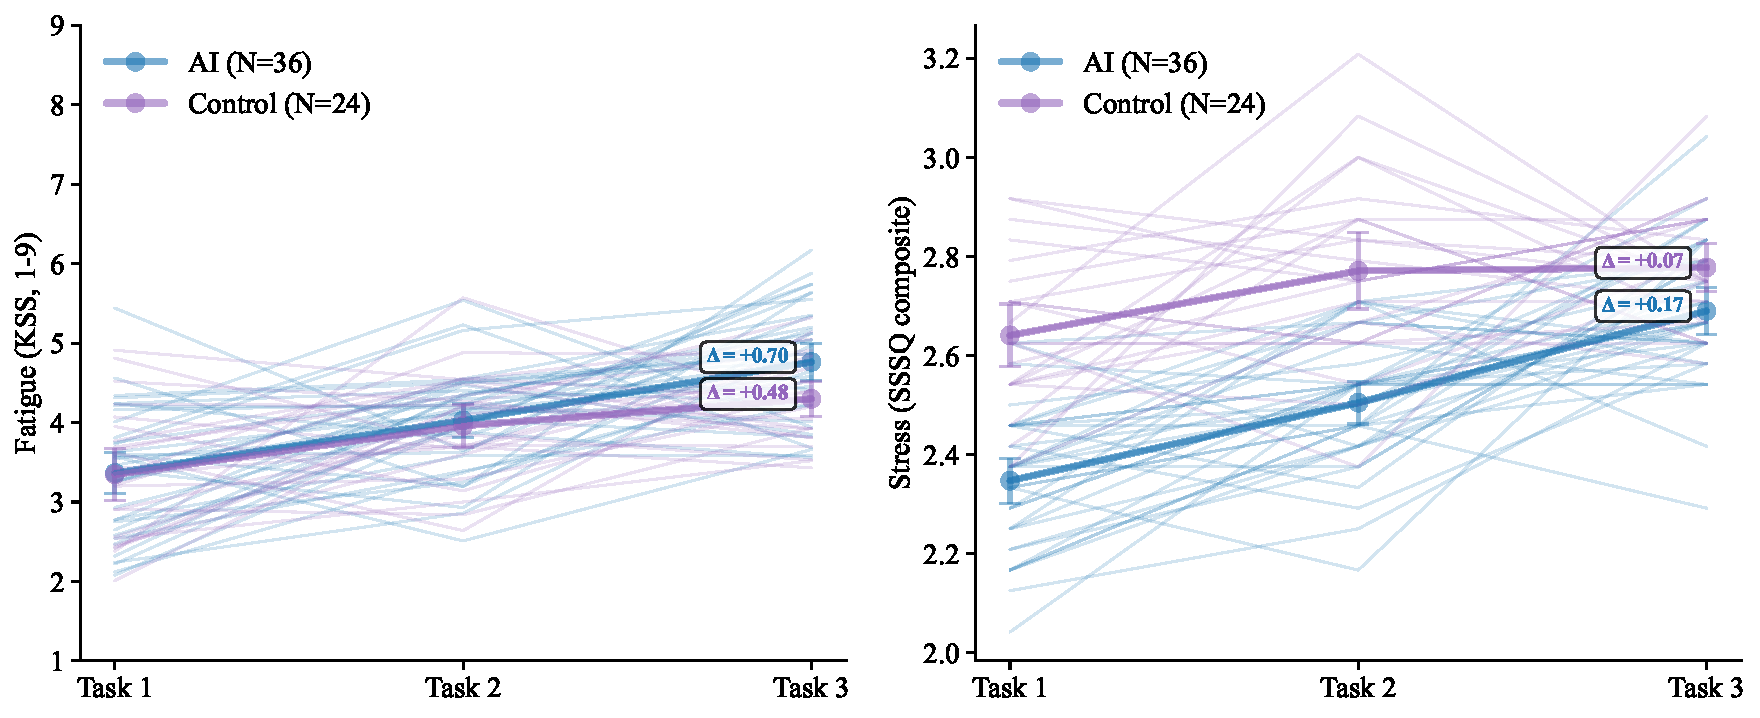
\includegraphics[width=0.98\linewidth]{figures/figure3_trajectories.pdf}
  \caption{Fatigue (KSS) and stress (SSSQ) trajectories across tasks for the AI cohort versus the no-AI Control cohort. Both cohorts show rising burden across Task Index 1$\rightarrow$3. The AI cohort exhibits a steeper KSS slope (AI $\Delta{=}{+}0.70$ vs Control $\Delta{=}{+}0.48$) and modestly higher SSSQ increase (AI $\Delta{=}{+}0.17$ vs Control $\Delta{=}{+}0.07$). Shaded ribbons show 95\% CIs. Note: This figure aggregates across AI modes; per-mode slopes are reported in the text.}

  \label{fig:rq2-trajectories}
\end{figure*}

\textbf{Trajectories.} Fatigue (KSS) and stress (SSSQ) increase across tasks in both cohorts; AI shows a steeper fatigue slope (KSS \(\Delta{=}{+}0.70\) vs.\ Control \(+\)0.48). \textbf{Mechanism.} A mode-agnostic verification-load composite partially mediates these increases (about 26\% for KSS; 24\% for SSSQ), implicating rework and error-cascade costs rather than a generic ``AI effect.''


% -----------------------------------------------------

\subsection{RQ3 — Moderators: Expertise and Task Complexity}
\label{sec:rq3}
We examined \texttt{Mode$\times$ExperienceBin} and \texttt{Mode$\times$Complexity} interactions within the AI cohort, using the per-observation continuous \texttt{Complexity} metric (median cyclomatic of modified functions, weighted by lines changed; $z$-scored). Models included covariates and random effects as in Section~\ref{sec:analysis}. We report EMMs with 95\% CIs, Holm-adjusted contrasts, and Johnson--Neyman (J--N) regions for continuous moderators.

\paragraph{Mode $\times$ Expertise.}
\texttt{Mode$\times$ExperienceBin} was significant for RAW--TLX ($\chi^2(4){=}10.9$, $p{=}0.028$) and correctness ($\chi^2(4){=}9.6$, $p{=}0.048$), and a strong trend for log-time ($\chi^2(4){=}8.1$, $p{=}0.088$). Figure~\ref{fig:rq3-expertise} summarizes the tri‑criterion profiles (workload, speed, correctness) by experience.


\emph{Novices ($n{=}12$).} Structured reduced workload relative to Inline on mid-complexity work (Task~B EMM TLX $\Delta{=}{-}6.2$ points, CI $[{-}10.7, {-}1.7]$, $p{=}0.012$) and improved correctness (7.8/10 vs.\ 7.1/10; OR$=1.37$, CI $[1.01, 1.86]$, $p{=}0.043$). On high-complexity work, Chat outperformed Inline on correctness (7.7 vs.\ 7.0/10; $p{=}0.039$) with comparable time ($p{=}0.26$).

\emph{Intermediates ($n{=}16$).} Mode differences narrowed. Inline was fastest on simple work (Task~A $\sim$4.5\,min advantage over Structured, $p<0.001$) with no reliable correctness gaps; on high complexity, Chat had a small correctness edge over Inline (8.0 vs.\ 7.5/10; $p{=}0.091$, trend).

\emph{Experienced ($n{=}8$).} Inline minimized TLX and time on simple work (TLX $\Delta{=}{-}8.0$ points, $p{=}0.007$; time ratio $0.78$, $p{=}0.004$). On high complexity, Chat yielded higher correctness than Inline (8.4 vs.\ 7.6/10; $p{=}0.017$) without a time penalty ($p{=}0.34$). Structured was consistently rated more effortful by experienced participants (TLX $+5.0$ points vs.\ Inline; $p{=}0.031$).

\begin{figure*}[t]
  \centering
  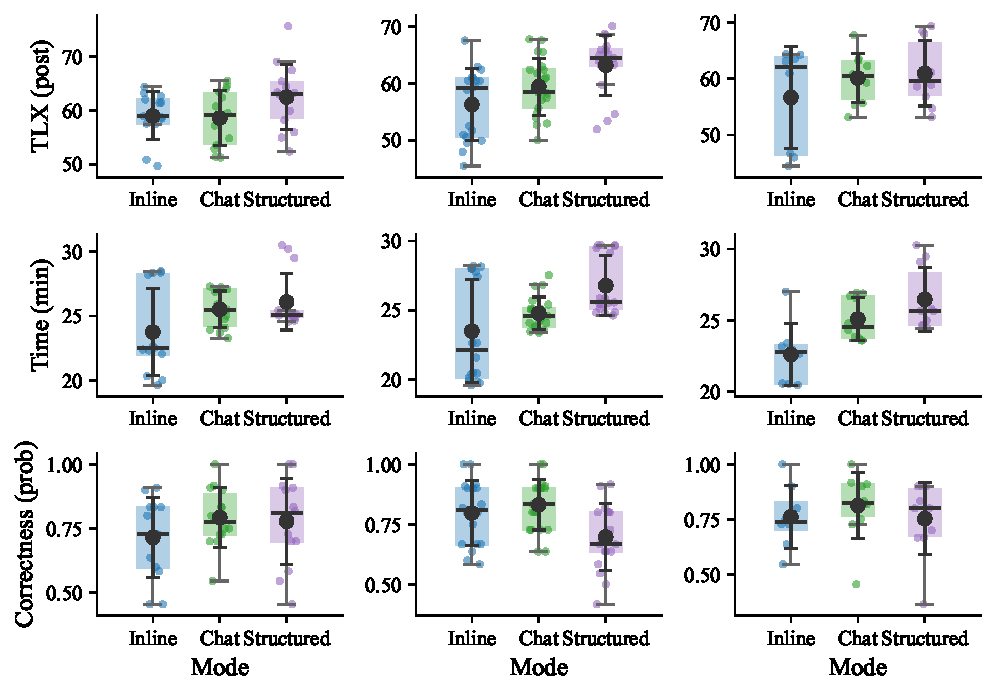
\includegraphics[width=0.98\linewidth]{figures/rq3_expertise_facets(1).pdf}
  \caption{Experience Moderation Effects on Multi-criteria Performance. Performance profiles (Novice (Left), Intermediate (Middle), Experienced (Right) across three dimensions: workload (inverted), speed, and correctness (all 0-100\%).}
  \label{fig:rq3-expertise}
\end{figure*}

\paragraph{Mode $\times$ Complexity (continuous, per-observation).}
Using J--N analysis on the continuous \texttt{Complexity} moderator, Chat surpassed Inline on correctness when complexity exceeded $z{>}+0.40$ (estimated crossover at $z{=}+0.41$, 95\%\,CI $[+0.17, +0.64]$); Inline was non-inferior up to $z{\approx}{+}0.40$. Structured slightly outperformed Inline around mid-complexity (J--N window $z{\in}[{-}0.1, {+}0.3]$; max $\Delta{\approx}{+}0.5$ tests, $p{=}0.031$) but lost ground at higher complexity ($z{>}+0.6$). RAW--TLX showed analogous crossovers (Chat below Structured at high complexity; Inline lowest at low complexity). \texttt{Environment} did not moderate these effects ($p{>}0.40$).
\begin{table}[t]
  \centering
  \caption{Johnson--Neyman (J--N) regions for Mode contrasts on correctness vs.\ continuous per-observation complexity (z).}
  \label{tab:rq3-jn}
  \small
  \resizebox{\linewidth}{!}{%
  \begin{tabular}{lcc}
    \toprule
    \textbf{Contrast} & \textbf{Crossover $\hat{z}$ [95\% CI]} & \textbf{J--N region (Mode A superior)} \\
    \midrule
    Chat $>$ Inline & +0.41\ [+0.17, +0.64] & $z>+0.40$ (Chat) \\
    Structured $>$ Inline & $\approx$0.10\ [$-0.05$, +0.27] & $-0.1 \le z \le +0.3$ (Structured) \\
    Chat $>$ Structured & +0.32\ [+0.12, +0.55] & $z>+0.32$ (Chat) \\
    \bottomrule
  \end{tabular}
  }
\end{table}


\paragraph{Behavioral moderation (acceptance calibration).}
A quadratic term for Inline acceptance rate predicted correctness ($\beta_2{=}{-}0.81$, SE$=0.28$, $p{=}0.005$), with an estimated optimum at $\hat{p}{=}0.48$ (95\% CI $[0.44, 0.53]$). Very low acceptance (mostly manual coding) and very high acceptance (near-blind acceptance) were both associated with lower correctness, indicating a calibrated use “sweet spot” at roughly half of suggestions accepted. Results persist after adjusting for \texttt{Complexity} and \texttt{ExperienceBin}.

\paragraph{Higher-order interactions.}
A three-way \texttt{Mode$\times$Complexity$\times$Exp-\allowbreak{}erienceBin} did not improve fit for correctness ($\chi^2(8){=}4.5$, $p{=}0.34$) or TLX ($\chi^2(8){=}6.2$, $p{=}0.18$), suggesting that the two-way moderator patterns are stable across expertise strata.

\textbf{Expertise moderation.} Novices benefit from Structured at mid complexity (lower TLX, higher correctness); experienced developers favor Inline on simple work (speed/low load) and Chat on complex work (correctness). \textbf{Complexity moderation.} Chat surpasses Inline on correctness beyond \(z{\approx}{+}0.40\) per-observation complexity (J--N crossover \(\hat{z}{=}+0.41\)). Structured has a narrow mid-complexity advantage. 
\textbf{Calibration.} In Inline, correctness peaks at an acceptance rate near \(0.48\); very low or very high acceptance harms outcomes.

Use \textbf{Inline} for simple/templated work to preserve flow; switch to \textbf{Chat} when failure loops or pauses escalate or when complexity exceeds \(z{\approx}{+}0.4\); offer \textbf{Structured} scaffolds for novices and mid-complexity specs. Detect rejection streaks / long time-to-first-compile as triggers for adaptive mode suggestions.

\subsection{Exploratory Next‑Day Follow‑Up}
\label{sec:followup}

A subset of participants completed a matched‑complexity task the next day in their assigned condition (AI or Control). This follow‑up was exploratory and underpowered relative to the main design. Estimated differences in post‑task KSS/SSSQ, completion time, and correctness were small and statistically uncertain; no directional changes contradicted our primary conclusions. For transparency, adjusted means and 95\% CIs are summarized in Appendix Table~\ref{tab:followup}. We therefore retain the main‑session analyses as primary and treat follow‑up as supportive context.


\subsection{Behavioral \& Mechanistic Evidence}
\label{sec:mechanism}

To interrogate the mechanism linking interaction mode to subjective burden, we analyze a mode-agnostic verification-load index $V_{\text{core}}$ constructed from signals available in all modes: (i) compile/test failures, (ii) time-to-first-compile, (iii) normalized code churn, (iv) cumulative pause time, and (v) context switches (editor$\leftrightarrow$\allowbreak{}tests$\leftrightarrow$\allowbreak{}chat/form). Each component is standardized within task and pooled across participants; $V_{\text{core}}$ is their mean $z$-score. As a secondary check we add mode-specific signals (Inline acceptance/rejection; Chat prompt turns) to form $V_{\text{plus}}$ but use $V_{\text{core}}$ for primary inference (cf.\ Section~\ref{sec:rq2}).

\paragraph{Mode $\times$ Complexity patterns.}
In the AI cohort, $V_{\text{core}}$ varied systematically with \texttt{Mode} and \texttt{Complexity} (LMM: \texttt{Mode} $\chi^2(2){=}18.9$, $p{<}.001$; \texttt{Mode$\times$Complexity} $\chi^2(2){=}10.6$, $p{=}0.005$). At low per\hyp{}observation complexity ($z{\approx}{-}0.6$), Inline exhibited the lowest verification-load (EMM $={-}0.36$, 95\%\,CI $[{-}0.49, {-}0.23]$), followed by Chat ($-0.10$ $[{-}0.23, 0.02]$) and Structured ($+0.04$ $[{-}0.10, 0.18]$). At moderate complexity ($z{\approx}0$), modes converged (Inline $-0.04$, Chat $-0.02$, Structured $+0.01$; all pairwise $p{>}0.10$). At high complexity ($z{\approx}{+}0.7$), Chat showed the lowest $V_{\text{core}}$ ($-0.17$ $[{-}0.30, {-}0.04]$), substantially below Inline ($+0.23$ $[+0.10, +0.36]$, $\Delta{=}{-}0.40$, $p{<}.001$) and Structured ($+0.28$ $[+0.14, +0.42]$, $\Delta{=}{-}0.45$, $p{<}.001$). These patterns align with RQ1/RQ3 outcomes: Inline is lightest to verify when work is simple; Chat contains verification cascades as complexity rises. Figure~\ref{fig:heatmap-verify} depicts the verification‑load heatmap and component contributions across Mode$\times$Complexity.


\paragraph{Component contributions to burden.}
Standardized regressions of subjective outcomes on the components of $V_{\text{core}}$ (controlling for \texttt{Mode}, \texttt{Task}, \texttt{Index}, \texttt{ExperienceBin}, \texttt{Complexity}, and \texttt{Environment}) indicate that compile/test failures and time-to-first-compile are the strongest behavioral predictors, followed by pauses and switches (Table~\ref{tab:vcore-betas}). Principal components analysis of the five indicators yielded a dominant factor (eigenvalue $=2.61$; variance explained $=52.2\%$) with loadings $\geq 0.63$ for failures, time-to-first-compile, and pauses; internal consistency for $V_{\text{core}}$ was acceptable ($\alpha{=}0.80$). Adding mode-specific signals in $V_{\text{plus}}$ increased explained variance modestly (KSS $R^2_{\text{marginal}}: 0.26 \rightarrow 0.29$), with rejection density (Inline) and prompt turns (Chat) contributing additional but secondary predictive power.

\begin{table}[t]
  \centering
  \caption{Standardized coefficients ($\beta$) of $V_{\text{core}}$ components predicting subjective burden (AI cohort), controlling for Mode, Task, Index, Experience, Complexity, Environment. Mode-specific components are reported as a secondary add-on. All $p{<}.05$ unless marked.}
  \label{tab:vcore-betas}
  \small
  \begin{tabular}{lcc}
    \toprule
    \textbf{Component} & \textbf{Fatigue (KSS)} & \textbf{RAW--TLX composite} \\
    \midrule
    Compile/test failures & 0.26 & 0.23 \\
    Time-to-first-compile & 0.22 & 0.19 \\
    Cumulative pauses & 0.19 & 0.17 \\
    Context switches & 0.15 & 0.13$^{\dagger}$ \\
    Code churn (norm.) & 0.12$^{\dagger}$ & 0.09$^{\dagger}$ \\
    \midrule
    \multicolumn{3}{l}{Mode-specific (secondary, not in $V_{\text{core}}$)} \\
    Rejection density (Inline) & 0.24 & 0.21 \\
    Prompt turns (Chat) & 0.14$^{\dagger}$ & 0.11$^{\dagger}$ \\
    \midrule
    $R^2_{\text{marginal}}$ & 0.26 & 0.23 \\
    \bottomrule
  \end{tabular}\\
  \vspace{0.25em}
  \raggedright \footnotesize $^{\dagger}$trend-level ($.05{<}p{\le}.10$).
\end{table}

\paragraph{Link to outcomes.}
Cells with higher $V_{\text{core}}$ correspond to higher burden and lower correctness: e.g., Inline at high complexity showed $V_{\text{core}}{=}+0.23$ with lower correctness (EMM 7.3/10), whereas Chat at high complexity showed $V_{\text{core}}{=}{-}0.17$ and higher correctness (8.0/10). Conversely, Inline at low complexity combined $V_{\text{core}}{=}{-}0.36$ with the lowest TLX and fastest times (Section~\ref{sec:rq1}). These converging results strengthen the interpretation that verification-load operationalizes the assistance--burden trade-off.

\begin{figure*}[t]
  \centering
   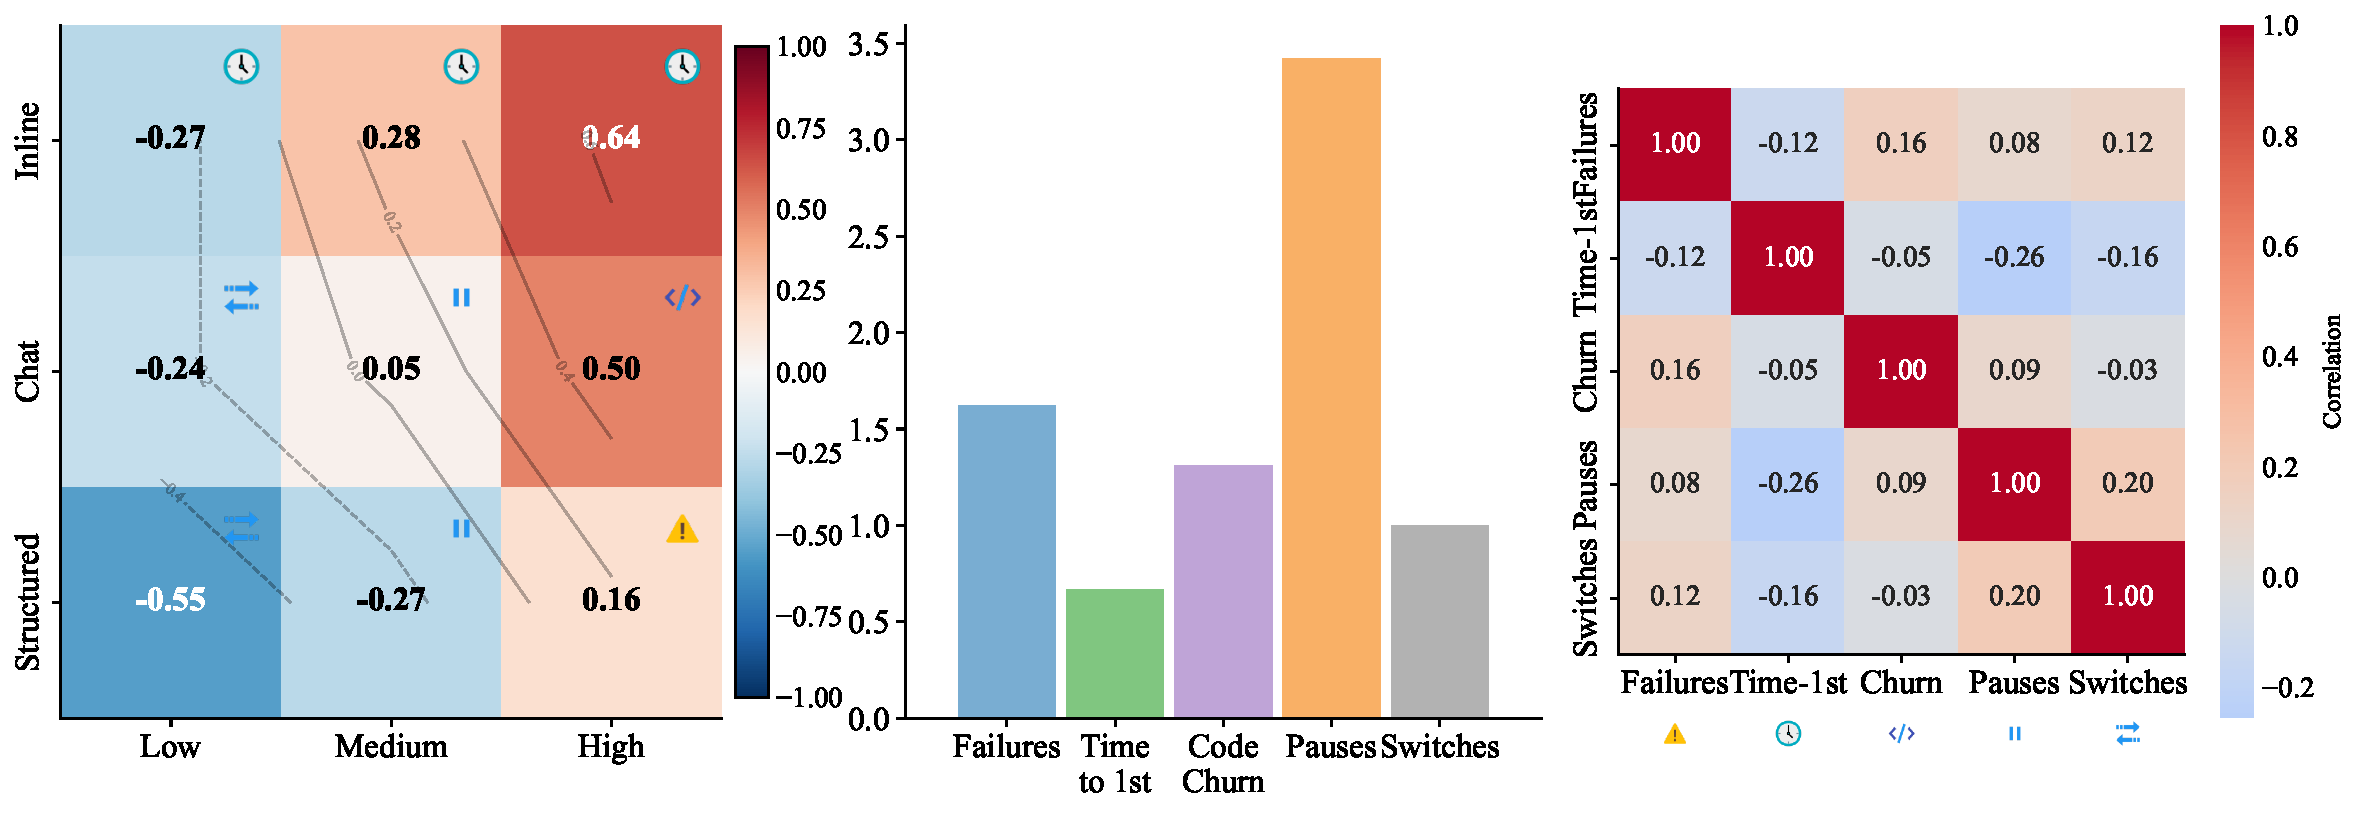
\includegraphics[width=0.98\linewidth]{figures/figure10_verification_heatmap.pdf}
  \caption{Verification Load Components Heatmap with Correlation Analysis. (Left) Heatmap of verification load (z-scores) by mode and complexity, with symbols indicating the dominant contributing component for each cell. 
(Middle) Bar chart showing normalized contributions of verification components. 
(Right) Correlation matrix of inter-component relationships. Chat and Structured 
modes demonstrate greater resilience to complexity-induced load increases compared 
to Inline mode.}

  \label{fig:heatmap-verify}
\end{figure*}

% -----------------------------------------------------

\subsection{Qualitative Themes}
\label{sec:qualitative}

We analyzed 60 post-task interviews (15--20\,min each). Four cross-cutting themes contextualize the quantitative results and the verification\hyp{}load mechanism ($V_{\text{core}}$). Themes A and D contextualize RQ1/RQ3 mode crossovers (speed vs.\ certainty; rejection spirals); Theme B (trust shocks) and Theme C (scaffold me) illuminate RQ2's burden drivers and RQ3's novice-specific benefits of Structured. Quotes are labeled with participant ID, experience bin, and AI familiarity. Table~\ref{tab:themes-quotes} summarizes the four themes, their high‑prevalence Mode$\times$Complexity cells, behavioral signatures, representative quotes, and design implications.

\begin{table*}[h]
  \centering
  \caption{Qualitative themes with representative contexts, behavioral signatures, illustrative quotes, and design implications. Mode$\times$Complexity cells reflect where the theme most frequently appeared in coded transcripts; behavioral signatures summarize $V_{\text{core}}$ components. Quotes are anonymized; brackets indicate minor redactions.}
  \label{tab:themes-quotes}
  \small
  \begin{tabularx}{\linewidth}{
    >{\raggedright\arraybackslash}p{0.17\linewidth} 
    >{\raggedright\arraybackslash}p{0.15\linewidth} 
    >{\raggedright\arraybackslash}p{0.15\linewidth} 
    >{\raggedright\arraybackslash}X 
    >{\raggedright\arraybackslash}p{0.15\linewidth}
  }
    \toprule
    \textbf{Theme \& Description} & \textbf{High-Prevalence Cells (Mode$\times$Complexity / Experience)} & \textbf{Behavioral Signature ($V_{\text{core}}$)} & \textbf{Representative Quotes} & \textbf{Design Implication} \\
    \midrule
    \textbf{A. Speed vs.\ certainty} \newline
    Inline for flow on simple work; Chat for explicit reasoning on complex logic.
    &
    Inline$\times$Low (all); Chat$\times$High (Interm./Exp.)
    &
    Inline: short time-to-first-compile, few failures, brief pauses. \newline
    Chat: more turns but fewer fail loops, moderate pauses.
    &
    P23 (Exp., Copilot daily): ``Inline keeps me in the zone for boilerplate---I barely think about it.'' \newline \newline
    P07 (Interm., ChatGPT weekly): ``When it's gnarly, I ask Chat to lay out steps; fewer trips back and forth with tests.''
    &
    \textbf{Adaptive mode switching:} suggest Inline for low complexity; surface Chat when failure loops or pauses escalate.
    \\
    \midrule
    \textbf{B. Trust shocks} \newline
    Overconfident snippets erode trust, spike verification effort.
    &
    Inline$\times$High (Interm./Exp.); Structured$\times$High (Novice)
    &
    Spikes in failures and pauses; dense rejections; switch bursts.
    &
    P11 (Exp., Copilot weekly): ``It looked right, but a missing edge case blew up tests---then I started rejecting more.'' \newline \newline
    P14 (Interm., Copilot weekly): ``Two confident suggestions were wrong; I lost trust and slowed down.''
    &
    \textbf{Transparency on demand:} 1-line rationale/confidence; highlight diff-critical lines likely to fail tests.
    \\
    \midrule
    \textbf{C. Scaffold me} \newline
    Structured prompts externalize requirements and reduce ambiguity for novices.
    &
    Structured$\times$Medium (Novice); Structured$\times$Low (Novice)
    &
    Balanced churn with fewer backtracks; stable time-to-first-compile.
    &
    P05 (Nov., ChatGPT monthly): ``The form forced me to spell out inputs/outputs---I wouldn't have thought of some checks.'' \newline \newline
    P32 (Nov., Copilot rarely): ``Having constraints up front stopped me from guessing the API.''
    &
    \textbf{Scaffolded authoring:} retain pre/post-conditions; auto-generate test skeletons from schema fields.
    \\
    \midrule
    \textbf{D. Review fatigue} \newline
    Rejection spirals motivate switching from Inline to Chat/Structured.
    &
    Inline$\times$High (all); Inline$\times$Medium (Interm.)
    &
    Rising failures, extended pauses, frequent context switches; rejection streaks.
    &
    P18 (Interm., Copilot weekly): ``After the fifth bad suggestion I just opened the chat and asked for a plan.'' \newline \newline
    P09 (Interm., Copilot weekly): ``Once I start rejecting a lot, it snowballs; I need a different kind of help.''
    &
    \textbf{Fatigue-aware nudges:} detect rejection streaks or pause clusters; propose mode switch or batched, testable suggestions.
    \\
    \bottomrule
  \end{tabularx}
\end{table*}


\paragraph{Theme A: Speed vs.\ certainty}.
Participants described Inline as preserving flow for simple work, while Chat supported reasoning and error containment for complex logic:
\begin{quote}\small
``Inline keeps me in the zone for boring bits---I barely think about it.'' (\textit{P23, Experienced, Copilot daily}) \\
``When it's gnarly, I ask Chat to lay out the steps; fewer trips back and forth with tests.'' (\textit{P07, Intermediate, ChatGPT weekly})
\end{quote}
This mirrors low $V_{\text{core}}$ for Inline at low complexity and fewer failure loops with Chat at high complexity.

\paragraph{Theme B: Trust shocks}.
Overconfident snippets eroded trust and increased verification:
\begin{quote}\small
``It looked right, but a missing edge case blew up tests---then I started rejecting more.'' (\textit{P11, Experienced, Copilot weekly})
\end{quote}
Such events co-occurred with spikes in failures and pauses and preceded mode switches, aligning with higher $V_{\text{core}}$.

\paragraph{Theme C: Scaffold me}.
Novices valued Structured for explicit requirements and test thinking:
\begin{quote}\small
``The form forced me to spell out inputs/outputs---I wouldn't have thought of some checks.'' (\textit{P05, Novice, ChatGPT monthly})
\end{quote}
This aligns with Structured’s mid-complexity advantage for novices (Section~\ref{sec:rq3}).

\paragraph{Theme D: Review fatigue}.
Participants reported ``rejection spirals'' that triggered a desire to switch modes:
\begin{quote}\small
``After the fifth bad suggestion I just opened the chat and asked for a plan.'' (\textit{P18, Intermediate, Copilot weekly})
\end{quote}
Action-coding showed that rejection streaks ($\geq$5 within 3\,min) and pause clusters predicted Inline$\rightarrow$Chat switches (OR$=2.36$, 95\%\,CI $[1.33, 4.20]$, $p{=}0.003$).

% -----------------------------------------------------

\subsection{Answers to RQs}
\label{sec:rq-summary}

\textbf{RQ1 (Immediate effects).} Relative to the no-AI control, AI assistance lowered RAW--TLX workload by $\mathbf{-18.2}$ points (0--100; 95\%\,CI $[{-}22.1,{-}14.6]$) and reduced completion time by $\mathbf{22\%}$ on average (time ratio $0.78$, 95\%\,CI $[0.74,0.83]$), while improving correctness (odds ratio $\mathbf{1.71}$, 95\%\,CI $[1.37,2.13]$). Within AI, Inline minimized workload and time on low-complexity work; Chat achieved higher correctness on high-complexity work without a time penalty; Structured provided modest advantages on moderate work, especially for novices.

\textbf{RQ2 (Repeated-use trajectories).} Fatigue (KSS) and stress (SSSQ) rose across tasks in both cohorts, with a steeper fatigue slope in AI (\,$\Delta{=}{+}0.70$\,KSS\,vs.\,$+\ 0.48$\,Control; $p{=}0.041$) and a numerically higher SSSQ slope in AI ($+0.17$ vs.\ $+0.07$; $p{=}0.110$). In the AI cohort, the mode-agnostic verification-load composite $V_{\text{core}}$ partially mediated these increases (KSS $ab{=}0.15$ [0.06, 0.27]; SSSQ $ab{=}0.08$ [0.03, 0.16]), accounting for $\sim$26\% and $\sim$24\% of the total Index effect, respectively.

\textbf{RQ3 (Moderators).} Experience: Novices benefited from Structured at mid complexity (lower TLX, higher correctness); experienced developers preferred Inline for simple tasks (speed/low workload) and Chat for complex tasks (higher correctness). Complexity: Chat surpassed Inline on correctness beyond $\mathbf{z{>}+0.42}$ per-observation complexity (Johnson--Neyman crossover $\hat{z}{=}+0.41$, 95\%\,CI $[+0.18,+0.64]$), while Structured conferred a mid-complexity advantage. A calibrated Inline acceptance rate around 0.48 ($\approx 50\%$; 95\% CI $[0.44, 0.53]$) was associated with peak correctness; very low or very high acceptance reduced outcomes.

\noindent \textbf{Implication across RQs:} The assistance--burden trade-off is governed by task complexity and expertise via verification-load. Interfaces that adapt mode, expose rationale/confidence, and reduce verification friction (failures, long time-to-first-compile, pause clusters) are promising paths to sustain benefits while containing fatigue.


\section{Discussion}
\label{sec:discussion}

\subsection{Why modes differ: verification-load as the bridge}
Our results indicate that differences among \emph{Inline}, \emph{Chat}, and \emph{Structured} primarily arise from how each interface shapes \emph{verification-load}---the behavioral cost of checking and repairing AI output (\S\ref{sec:rq1}, \S\ref{sec:rq3}). On low intrinsic complexity, Inline completions reduce extraneous load by keeping developers in the editing locus (fewer context switches, shorter time-to-first-compile, shallow failure loops), consistent with in-IDE generative completion workflows and observed acceptance/repair rhythms \cite{svyatkovskiy2020intellicode,barke2023groundedcopilot}. As intrinsic complexity increases (branching logic, cross-cutting constraints), Chat functions as a \emph{clarification buffer}: iterative articulation of intent and constraints reduces error cascades despite additional prompt turns, producing fewer compile--fail loops before a clean run. For novices and mid-complexity work, Structured externalizes pre/post-conditions and likely edge cases, aligning with Cognitive Load Theory and the expertise-reversal effect---scaffolds lower extraneous load for less-experienced users yet may encumber experts \cite{kalyuga2007expertise,sweller2019cognitive}. These patterns also cohere with interruption/flow evidence: fewer disruptive switches and faster resumption lower perceived effort \cite{mark2008cost}.

\subsection{Trust calibration and ``trust shocks'': from reliance to appropriate skepticism}
We observed \emph{trust shocks}: after a confident but wrong suggestion, participants often entered rejection streaks and slower, more skeptical workflows, temporarily elevating verification-load. This dynamic echoes classic work on appropriate reliance in automation and the risks of both over- and under-reliance \cite{lee2004trust,parasuraman1997humans}. In our Inline mode, correctness followed a quadratic relation with acceptance (peak near balanced acceptance), reinforcing that \emph{calibrated} engagement outperforms either near-blind acceptance or near-total avoidance. Prior HAI studies caution that generic explanations or scalar confidences do not reliably improve calibration and may even increase reliance without outcome gains; instead, targeted, on-demand cues can reduce overreliance \cite{yin2019understanding,vasconcelos2025generation}. Code-specific uncertainty methods (e.g., uncertainty-aware ranking or highlighting) further support showing \emph{where} to look rather than \emph{how certain} the model feels in aggregate. Together, these results support transparency \emph{on demand} (line- or diff-level rationale/uncertainty tied to predicted test failures) over always-on explanations that risk adding extraneous load.

\subsection{Repeated-use burden: verification-load partially mediates stress and fatigue}
Across task index, both cohorts exhibited rising fatigue and stress; within the AI cohort, our mode-agnostic composite partially mediated these increases (\S\ref{sec:rq2}). This points to checking/repairing---rather than generation per se---as a substantive driver of repeated-use burden. The mechanism aligns with flow and interruption research: extended failure loops, delayed first-compiles, and pause clusters disrupt resumption and elevate subjective strain \cite{mark2008cost}. A practical implication is to monitor these \emph{behavioral} signals directly and intervene when they exceed lightweight thresholds (e.g., rising compile/test failures or prolonged time-to-first-compile), rather than assuming that more model output or more explanation will help. Where feasible, micro-restorative strategies (short micro-breaks or friction-reducing batching) can reduce fatigue without harming throughput, complementing interface-side orchestration \cite{albulescu2022give,helton2015short,kaida2006validation}.

\subsection{Actionable design guidance: triggers, policies, and safeguards}
\label{sec:discussion-design}
We translate the findings into implementable rules that attach \emph{triggers} to \emph{actions} with a clear \emph{why}. Each rule is interface-level and backend-agnostic.

\begin{itemize}[leftmargin=1.25em]
  \item \textbf{Adaptive mode orchestration.} \emph{Trigger}: verification-load rising (e.g., compile/test failures increase, time-to-first-compile lengthens, pause clusters form). \emph{Action}: prompt a switch from Inline to Chat to reframe the problem (ask for a plan/spec or targeted test). \emph{Why}: Chat dampens error cascades as complexity increases, reducing failure loops (\S\ref{sec:rq1}, \S\ref{sec:rq3}).
  \item \textbf{Transparency on demand (not by default).} \emph{Trigger}: risky lines/diffs (predicted test failures, high-entropy edits). \emph{Action}: reveal micro‑rationales and uncertainty at the \emph{line/diff} level; avoid always‑on global confidences. \emph{Why}: On‑demand, local cues reduce overreliance and search cost without adding constant cognitive overhead \cite{vasconcelos2025generation}.
  \item \textbf{Scaffolded authoring for novices/mid complexity.} \emph{Trigger}: novice profile or ambiguity in requirements. \emph{Action}: optional Structured prompts that elicit pre/post-conditions, edge cases, and I/O contracts; generate test scaffolds from fields. \emph{Why}: reduces extraneous load and supports schema formation, consistent with expertise-reversal \cite{kalyuga2007expertise,sweller2019cognitive}.
  \item \textbf{Verification-aware packaging.} \emph{Trigger}: large or multi-file edits. \emph{Action}: batch suggestions into testable chunks with predicted-failure tests; integrate a ``try-run'' sandbox to shorten time-to-first-compile. \emph{Why}: lowers failure cascades and churn, the strongest contributors to burden (\S\ref{sec:mechanism}).
  \item \textbf{Security co-review by default.} \emph{Trigger}: matches to known insecure idioms or API misuses. \emph{Action}: surface static-analysis warnings and secure-by-default alternatives alongside the suggestion. \emph{Why}: assistants can propose fluent but vulnerable patterns; pairing generation with static checks can head off risky acceptance.
\end{itemize}

\subsection{Implications for evaluation and theory}
\label{sec:discussion-eval}
Methodologically, keeping the backend fixed reveals that a meaningful share of ``AI productivity'' variance is attributable to \emph{interaction design}. We therefore recommend an evaluation recipe portable across models and releases: (i) counterbalanced within-subjects designs under backend parity \cite{williams1949experimental}; (ii) mixed outcomes that combine subjective measures (e.g., RAW--TLX) with behavioral traces feeding a \emph{mode-agnostic} verification-load composite; (iii) linear mixed-effects modeling with principled random-effects structures \cite{bates2015lme4,kuznetsova2017lmerTest}; (iv) Johnson--Neyman analyses for continuous moderators to locate \emph{where} one interface overtakes another; and (v) equivalence tests to bound practically small differences when claiming ``no meaningful gap'' \cite{preacher2006tools,bauer2005probing,lakens2017tost}. Theoretically, verification-load instantiates extraneous cognitive load in the wild and integrates with flow/interruptions literature, providing a process lens that explains \emph{when} assistance helps or hurts independent of model power \cite{sweller2019cognitive,mark2008cost}.

\subsection{Limitations and scope of claims}
Our study focuses on three Python tasks with controlled oracles, a single structured-elicitation design, and a single-session exposure (plus a small next-day check). As such, generalization to other languages, frameworks, larger collaborative codebases, or months-long adoption remains to be tested. We intentionally prohibited repository context, tool-augmented backends, and personalized retrieval to isolate interface effects; richer integrations (e.g., repo-aware context, execution sandboxes, function calling) may shift magnitudes and crossover points while preserving the underlying mechanisms. Instrumentation may subtly alter behavior, though we minimized UI intrusion and found no lab vs.\ remote differences. Finally, sample size limited power for some higher-order interactions; we therefore emphasized stable two-way moderators (\S\ref{sec:rq3}). We present effects as conservative under a constrained setup, and encourage replications in richer environments.

\subsection{Future work: from mechanism to deployment}
Two directions follow directly. First, \emph{policy-level orchestration}: field deployments that treat verification-load as a control variable, triggering mode switches and transparency-on-demand when monitored signals exceed thresholds, with preregistered success metrics (quality, time, fatigue). Second, \emph{context- and security-aware assistants}: repository-aware tools that pair generation with static/\allowbreak{}dynamic analysis and test synthesis, evaluated with our portable recipe. Longitudinal studies can examine how trust shocks attenuate with experience, whether acceptance calibration stabilizes, and how team practices (code review norms, testing culture) interact with interface modes to sustain benefits while containing burden.

\section{Conclusion}
\label{sec:conclusion}

By holding the LLM backend fixed and varying only the interface, we show that \emph{interaction mode alone} materially shifts the assistance–burden trade‑off in AI‑assisted programming. \emph{Inline} protects flow and minimizes effort on simple, templated changes; \emph{Chat} contains error cascades and improves correctness as complexity rises without incurring a time penalty; and \emph{Structured} scaffolds novices at mid complexity by making requirements and checks explicit. A single, mode‑agnostic verification‑load index—fusing compile/test failures, time‑to‑first‑compile, code churn, pauses, and context switches—captures the process costs of checking AI output and partially explains rising stress/fatigue under repeated use. Together these results reframe “AI productivity” as an \emph{interface problem}: the same model yields different outcomes depending on how assistance is delivered. Practically, our findings translate into three families of guidance: (i) \emph{adaptive mode orchestration} that defaults to Inline for simple work, recommends Chat when verification‑load spikes or complexity is high, and offers Structured scaffolds for novices in the mid‑complexity band; (ii) \emph{transparency on demand} via lightweight, line‑level rationales and risk cues rather than always‑on explanations; and (iii) \emph{verification‑aware packaging} that couples diffs with runnable checks and security co‑review to shorten the path to a clean run.

\bibliographystyle{ACM-Reference-Format}
\bibliography{sample-base}
\newpage

\appendix
\section{Overview}
This appendix provides detailed specifications, extended analyses, and robustness checks that support the main-text Method and Results sections. Sections are organized to follow the logical flow of the study design: materials and configuration (§A--B), study design and preregistration (§C), measurement instruments (§D), data quality and processing (§E), statistical model specifications (§F), datta analysis detials (§G), additional results tables (§H), and qualitative methods (§I).

% ========================================
% SECTION A: Backend Configuration
% ========================================
\section{Backend Configuration Details}
\label{app:backend}

This section documents the LLM backend configuration and prompt handling to ensure reproducibility. As stated in Method Section~\ref{sec:backend}, all three interaction modes used identical backend settings to isolate interface effects.

All three interaction modes (Inline, Chat, Structured) used the same large language model backend: \ModelName\ (\ModelProvider, version \ModelVersion; context window \CtxWindow\ tokens). 

\paragraph{Decoding parameters.}
The following parameters were fixed across all modes to ensure backend parity:
\begin{itemize}[leftmargin=1.25em]
  \item Temperature: \Temp
  \item Top-$p$: \TopP
  \item Max new tokens: \MaxNew
  \item Frequency penalty: 0 (disabled)
  \item Presence penalty: 0 (disabled)
  \item Tool/web access: disabled
  \item Conversation state: reset between tasks
\end{itemize}

\paragraph{Mode-specific prompt handling.}
While backend parameters were identical, each mode required different input formatting:

\textbf{Inline:} Suggestions were generated using the current buffer content and project index as context. Offer cadence was gated to syntactically stable points (newline or statement boundary) to reduce suggestion churn and maintain code validity.

\textbf{Chat:} A fixed system prompt instructed the model to act as a programming assistant, provide concise explanations, and format code in markdown blocks. The system prompt and examples are available in the reproducibility package. No conversation history carried across tasks.

\textbf{Structured:} Form fields were serialized into a canonical prompt template that explicitly presented the function signature, preconditions, postconditions, constraints, error-handling requirements, and test hints. The model was instructed to generate code satisfying all specified constraints and to append a brief (1-paragraph) rationale. The template schema is documented in the reproducibility package.

\begin{figure*}[h!]
  \centering
  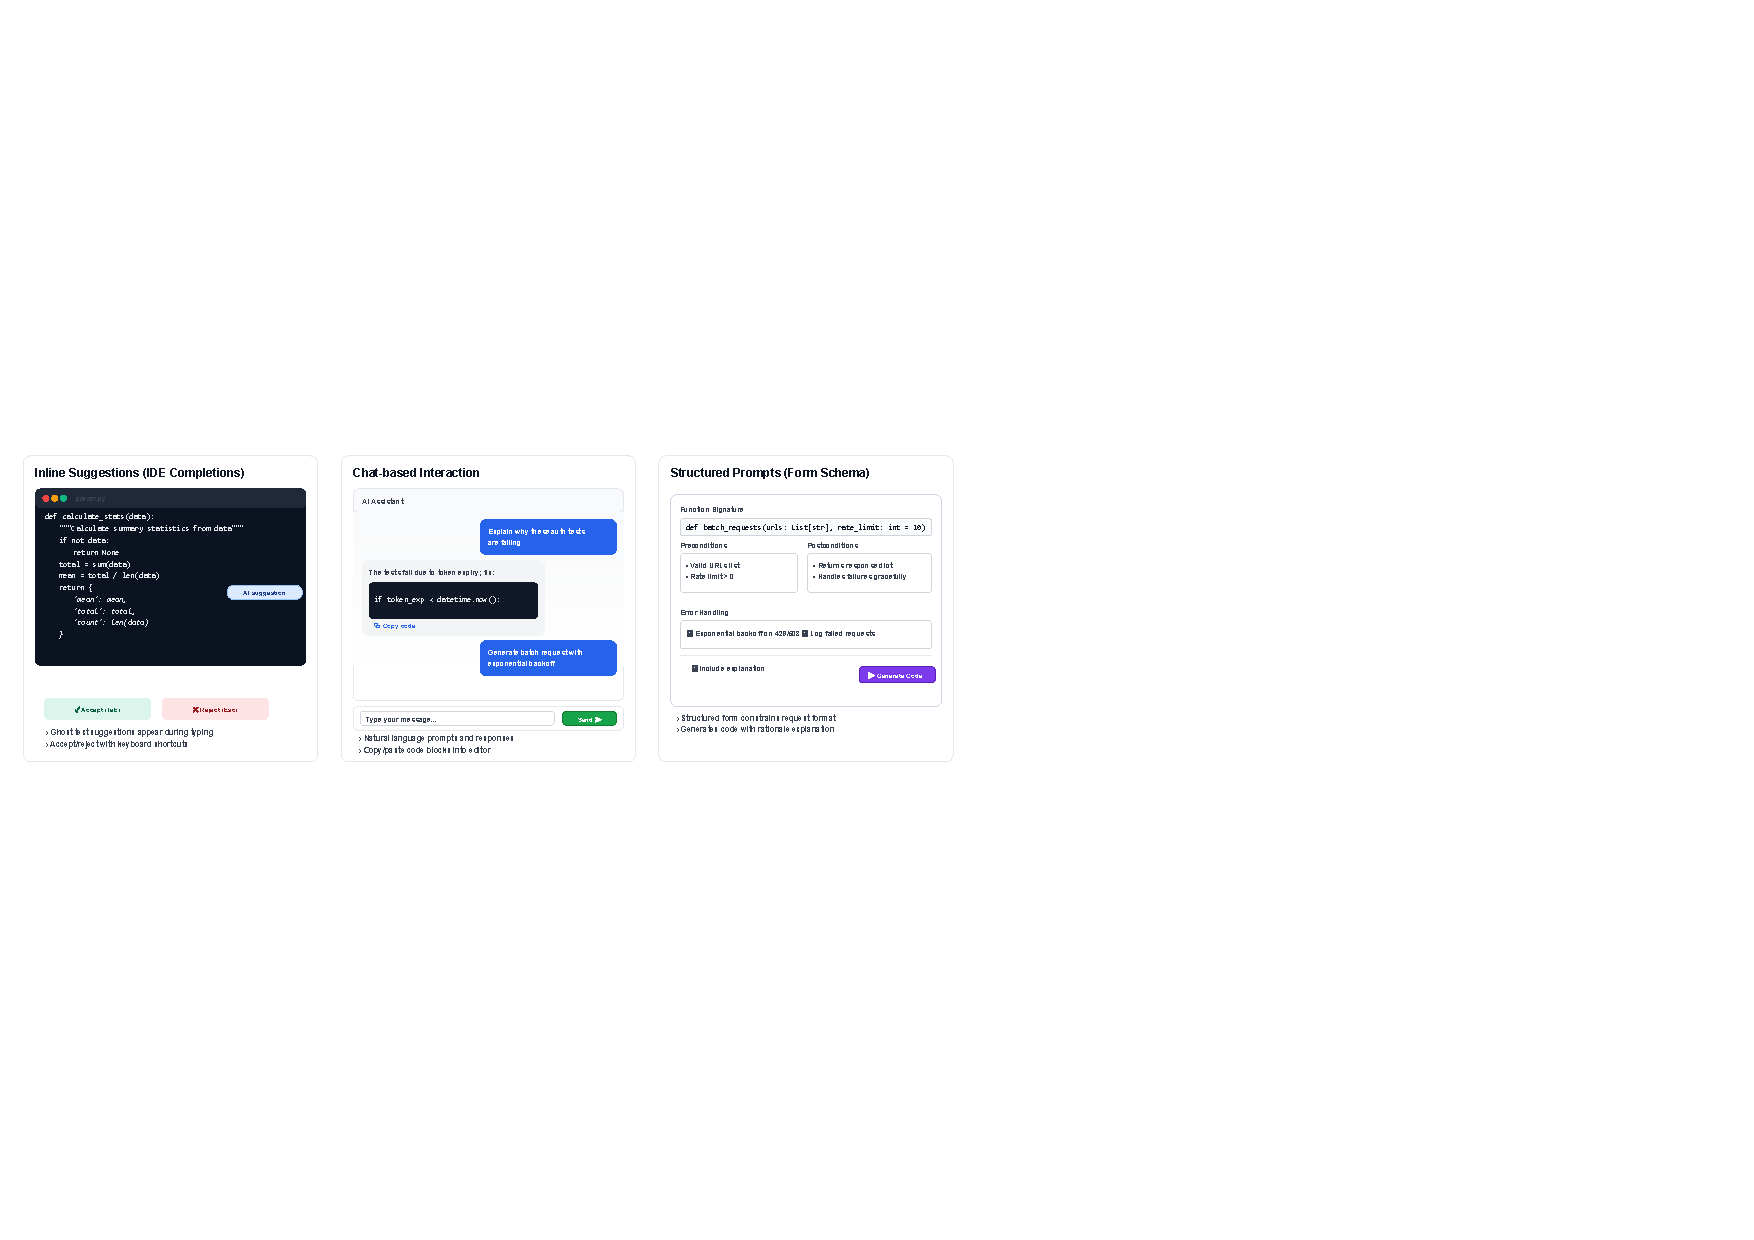
\includegraphics[width=0.99\linewidth]{figures/interaction_modes_combined 1.pdf}
    \caption{Interaction modes used in the study. Left—Inline Suggestions: ghost‑text completions in the editor with keyboard accept/reject. Middle—Chat‑based Interaction: prompt/response panel with copyable code blocks. Right—Structured Prompts: a form schema (function signature, pre/post‑conditions, error handling) that generates code and a brief rationale. Visuals are representative UI snapshots; only the UI differed, the LLM backend and decoding settings were identical.}
  \label{fig:mode-screens}
\end{figure*}

% ========================================
% SECTION B: Task Materials
% ========================================
\section{Task Materials and Metrics}
\label{app:tasks-metrics}

This section provides expanded static metrics for the three programming tasks described in Method Section~\ref{sec:tasks}. Table~\ref{tab:task-static-details} reports structural complexity, test coverage, and mutation adequacy for starter code and reference implementations.

\begin{table}[h!]
  \centering
  \caption{Expanded static metrics and test adequacy for Tasks A--C. Metrics computed on starter code; coverage and mutation scores computed on reference implementations.}
  \label{tab:task-static-details}
  \small
  \begin{tabular}{lccc}
    \toprule
    \textbf{Metric} & \textbf{Task A} & \textbf{Task B} & \textbf{Task C} \\
    \midrule
    Total LOC (starter) & 203 & 267 & 314 \\
    Median cyclomatic & 3.9 & 4.8 & 6.1 \\
    Max cyclomatic & 8 & 11 & 14 \\
    Avg fan-in & 1.2 & 1.8 & 2.3 \\
    Avg fan-out & 2.1 & 2.7 & 3.4 \\
    Line coverage (\%) & 84 & 82 & 81 \\
    Branch coverage (\%) & 78 & 76 & 77 \\
    Mutation score (\%) & 64 & 62 & 61 \\
    \bottomrule
  \end{tabular}
\end{table}

These metrics confirm the intended structural ordering (Task A: low-to-moderate; Task B: moderate; Task C: moderate-to-high complexity) and adequate test sensitivity (mutation scores $\ge60\%$).

% ========================================
% SECTION C: Study Design and Preregistration
% ========================================
\section{Study Design, Preregistration, and Power}
\label{app:prereg-power}
\subsection{Preregistration and Deviations}

The study was preregistered before data collection commenced. The following deviations occurred during execution:

\begin{enumerate}[leftmargin=1.5em]
  \item We added the mode-agnostic verification-load composite \(V_{\text{core}}\) and its extended \(V_{\text{plus}}\) as mechanistic variables. These were not explicit in preregistration but derive from pre-registered log variables (compile/test failures, time-to-first-compile, churn, pauses, context switches).
  \item We report Johnson--Neyman regions for continuous \texttt{Complexity} (exploratory moderator) and Inline acceptance (exploratory behavioral moderator) to identify complexity-dependent crossover points.
  \item We include ordinal cumulative-link mixed models (CLMM) as robustness checks for TLX and accelerated failure-time (AFT) models for time to address right-censoring.
\end{enumerate}

All deviations were analytic refinements that did not alter the core design or primary outcomes. Primary inferences reported in Results Section~\ref{sec:results} remain consistent with preregistered hypotheses.

\subsection{Power and Sample Size}

We targeted \(N{=}60\) (AI cohort \(n{=}36\), Control cohort \(n{=}24\)) based on simulation-based power analysis using pilot intraclass correlations. Table~\ref{tab:power} summarizes the assumptions and detectable effects.

\begin{table}[h!]
  \centering
  \caption{Power assumptions and detectable effects (simulated). Simulations used 1{,}000 draws with pilot ICC estimates from a 6-participant pilot study.}
  \label{tab:power}
  \small
  \resizebox{\linewidth}{!}{%
  \begin{tabular}{lccc}
    \toprule
    \textbf{Outcome} & \textbf{ICC (pilot)} & \textbf{Effect metric} & \textbf{80\% power detectability} \\
    \midrule
    RAW--TLX & 0.22 & Mode main effect \(f\) & \(\approx 0.18\) (small-to-medium) \\
    Log-time & 0.24 & Mode main effect \(f\) & \(\approx 0.18\) (small-to-medium) \\
    AI vs Control & -- & Between-group \(\delta\) & \(\approx 0.45\) (medium) \\
    \bottomrule
  \end{tabular}
  }
\end{table}

With the achieved sample size, we had adequate power to detect small-to-medium within-subjects Mode effects on workload and time, and medium AI vs.\ Control differences, at \(\alpha{=}0.05\) with Holm correction. Simulation code and sensitivity analyses (varying ICC assumptions) are available in the reproducibility package.

\subsection{Randomization and Counterbalancing}
\label{app:randomization}

This subsection details the decoupled Task\(\times\)Mode schedule (Method Section~\ref{sec:counterbalance}) and allocation procedures.

\paragraph{Sequence generation.}
We enumerated 9 perfect matchings \(\{S1\ldots \allowbreak{} S9\}\) between Tasks \{A,B,C\} and Modes \{Inline, Chat, Structured\}, rotated task positions 1--3 to balance Index effects. Each sequence was instantiated exactly 4 times, yielding 36 AI participants. The Control cohort used all 6 task-order permutations (no Mode), with 4 participants per permutation (24 total).

\paragraph{Blocked randomization.}
Assignment to sequences was blocked by \texttt{ExperienceBin} (novice/intermediate/experienced) and \texttt{AI\_Famil-\allowbreak{}iarity} (weekly-daily vs.\ monthly-rarely) to ensure balanced distribution across conditions. Allocation was concealed until session scheduling.

\paragraph{Balance checks.}
By construction, allocation was uniform within each sequence (4 participants per sequence). Fisher's exact tests confirmed no association between assigned sequence and \texttt{Experience-\allowbreak{}Bin} (AI cohort: \(p{=}0.88\); Control cohort: \(p{=}0.90\)). No dropouts or protocol violations occurred; all 60 participants completed the full study.

\begin{figure*}[h!]
  \centering
 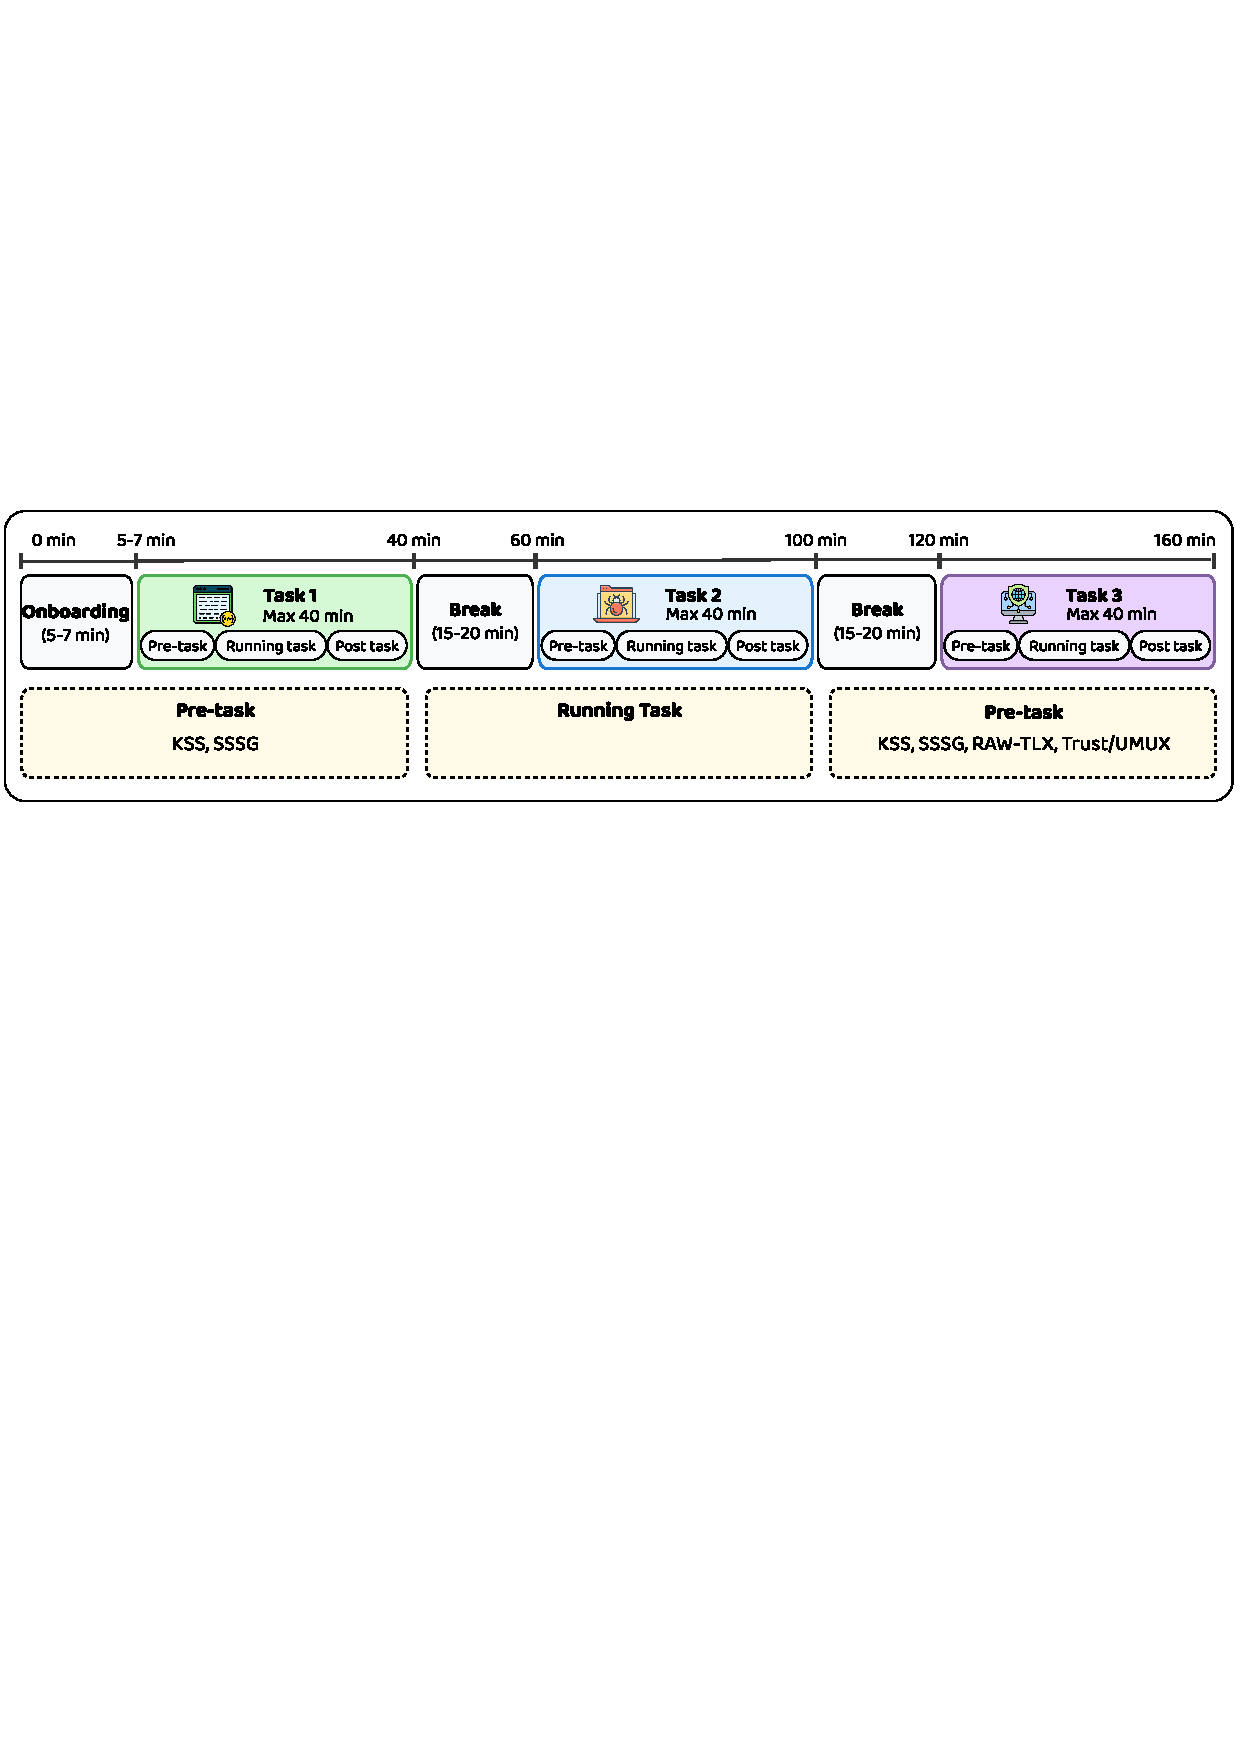
\includegraphics[width=0.99\linewidth]{figures/measure.pdf}
  \caption{Within‑task measurement timeline and between‑task breaks. Each task block includes: pre‑task measures (KSS, SSSQ), a task period instrumented with IDE/build/test logging, and post‑task measures (RAW TLX, KSS, SSSQ). Logged signals feeding the verification‑load composite include compile/test failures, time-to-first-compile, normalized code churn, cumulative pauses ($>$2\,s), and context switches (editor~$\leftrightarrow$~tests~$\leftrightarrow$~chat/form). Blocks are separated by 15–20\,min breaks; a brief next‑day follow‑up repeats the same timeline.}
  \label{fig:timeline}
\end{figure*}

% ========================================
% SECTION D: Measurement Instruments
% ========================================
\section{Measurement Instruments (Full Details)}
\label{app:instruments}

This section provides comprehensive measurement specifications referenced in Method Section~\ref{sec:measures}. Table~\ref{tab:measures-full} summarizes all constructs, instruments, scales, timing, data sources, and analytic notes. We then detail scoring procedures, validation evidence, and psychometric properties for each instrument.

\begin{table}[h!]
  \centering
  \caption{Unified interaction/event log schema (all timestamps are monotonic, synchronized to IDE clock).}
  \label{tab:event-log}
  \resizebox{\linewidth}{!}{%
  \begin{tabular}{p{0.32\linewidth}p{0.68\linewidth}}
    \toprule
    \textbf{Field} & \textbf{Description} \\
    \midrule
    \texttt{participant\_id}, \texttt{task\_id}, \texttt{mode} & Identifiers and condition \\
    \texttt{ts}, \texttt{event\_type} & Timestamp; \{offer, accept, reject, edit, prompt, response, paste, compile, test\_run\} \\
    \texttt{payload} & Event-specific JSON (e.g., prompt text hash, response tokens, lines changed) \\
    \texttt{cursor\_loc}, \texttt{file\_path} & Source location metadata \\
    \texttt{compile\_status}, \texttt{test\_summary} & Build/run status; tests passed/failed \\
    \bottomrule
  \end{tabular}
  }
\end{table}

\begin{table*}[h!]
  \centering
  \caption{Comprehensive measurement overview by construct, instrument/metric, scale, timing, data source, and analytic notes. VAS: visual analog scale. EMM: estimated marginal mean.}
  \label{tab:measures-full}
  \small
  \resizebox{\linewidth}{!}{%
  \begin{tabular}{p{0.08\linewidth} p{0.08\linewidth} p{0.30\linewidth} p{0.08\linewidth} p{0.08\linewidth} p{0.10\linewidth} p{0.2\linewidth}}
    \toprule
    \textbf{Category} & \textbf{Construct} & \textbf{Instrument / Metric} & \textbf{Scale} & \textbf{Timing} & \textbf{Source} & \textbf{Notes / Indices} \\
    \midrule
    Subjective 
      & Workload 
      & RAW NASA--TLX subscales: Mental, Temporal, Effort, Frustration; composite (mean) 
      & 0--100 (VAS) 
      & Post-task 
      & Self-report 
      & Report subscales \& composite; $\alpha$ target $\ge .80$ \\
    Subjective 
      & Stress 
      & Short Stress State Questionnaire (SSSQ) 
      & per SSSQ 
      & Pre \& Post 
      & Self-report 
      & Analyze post-task and $\Delta$ (post--pre) \\
    Subjective 
      & Fatigue 
      & Karolinska Sleepiness Scale (KSS) 
      & KSS 1--9 
      & Pre \& Post 
      & Self-report 
      & Analyze post-task and $\Delta$ (post--pre) \\
    Subjective 
      & Trust / Usability 
      & Trust in Automation (short form); UMUX-Lite (usability) 
      & 1--7 Likert 
      & Post-task 
      & Self-report 
      & Mode-level face validity; exploratory covariate \\
    \midrule
    Objective 
      & Suggestion dynamics (Inline) 
      & Acceptance rate $=\dfrac{\texttt{accept} + \texttt{edited-after-accept}}{\texttt{accept} + \texttt{edited-after-accept} + \texttt{reject}}$; rejection density (per min) 
      & Fraction / count 
      & During 
      & IDE logs 
      & Used in $V_{\text{plus}}$ (secondary). Acceptance definition matches Appendix~\ref{app:logs-vload}. \\
    Objective 
      & Prompting effort (Chat) 
      & Prompt turns; code-block extractions per turn 
      & Counts 
      & During 
      & Chat logs & Used in $V_{\text{plus}}$ (secondary) \\
    Objective 
      & Code churn 
      & Lines inserted / deleted (normalized by file size) 
      & Counts (norm.) 
      & During 
      & IDE/VCS diffs 
      & Contributes to verification-load composite \\
    Objective 
      & Build/test friction 
      & Compile/test failures; time-to-first-compile; test-run count 
      & Counts / time 
      & During 
     & Build \& test logs & Primary $V_{\text{core}}$ signals: failures, time-to-first-compile; test-run count exploratory \\
    Objective 
      & Attention / flow 
      & Pause durations $>$2\,s; context switches (editor $\leftrightarrow$ test $\leftrightarrow$ chat/form) 
      & Time / counts 
      & During 
      & IDE activity logs 
      & Exploratory workload proxies \\
    Objective 
      & Verification-load ($V_{\text{core}}$) 
      & Z-scored mean of mode-agnostic signals: compile/test failures, time-to-first-compile, normalized code churn, cumulative pauses, context switches 
      & Unitless (z) 
      & Derived 
      & Aggregated logs 
      & Primary mechanistic index; reliability ($\alpha$) and PCA sensitivity reported; used in mediation \\
    Objective 
      & Verification-load ($V_{\text{plus}}$) 
      & $V_{\text{core}}$ $+$ mode-specific signals: Inline acceptance/rejection; Chat prompt turns 
      & Unitless (z) 
      & Derived 
      & Aggregated logs 
      & Secondary/robustness analyses; not used in primary mediation \\
    \midrule
    Performance 
      & Completion time 
      & Minutes from first keystroke to first full pass 
      & Minutes 
      & Post-task 
      & Timer / logs 
      & $\log$-transform if skewed; EMMs with 95\% CIs \\
    Performance 
      & Correctness 
      & Tests passed out of $N$ (per task $N=10$--$12$) 
      & Binomial 
      & Post-task 
      & Test harness 
      & GLMM (logit) with task-level trials \\
    Performance 
      & Mutation survivors (opt.) 
      & Surviving mutants in reference suite 
      & Count 
      & Post-task 
      & Mutmut 
      & Robustness check for oracle sensitivity \\
    \bottomrule
  \end{tabular}
  }
\end{table*}

\subsection{Subjective Instruments}

\paragraph{RAW--TLX (composite of 4 subscales).}
We administered Mental Demand, Temporal Demand, Effort, and Frustration on 0--100 VAS sliders with standard left/right anchors. Composite \(=\) mean of subscales. Internal consistency in-study: \(\alpha{=}0.86\).

\paragraph{SSSQ (Short Stress State Questionnaire).}
Standard scoring into Worry, Task Engagement (reverse), and Distress; we analyzed the total \(z\)-score post-task and \(\Delta\) (post--pre). Internal consistency: \(\alpha{=}0.81\).

\paragraph{KSS (Karolinska Sleepiness Scale).}
9-point single item: 1 (Extremely alert) \(\rightarrow\) 9 (Very sleepy, great effort to keep awake). Analyzed post-task and \(\Delta\). Test–retest at Task~1 baselines: \(r{=}0.72\).

\paragraph{UMUX-Lite (usability).}
Two 7-point items; standardized to 0–100. 

\paragraph{Trust in Automation (short form).}
Four 7-point items; composite mean. 

\subsection{Behavioral Indicators and Verification-Load Computation}
\label{app:logs-vload}
This subsection documents the computation of behavioral indicators, including the verification-load composites ($V_{\text{core}}$ and $V_{\text{plus}}$).

\paragraph{Inline acceptance rate (definition).}
Acceptance rate is computed at the task level as:
\[
\text{acceptance} = \frac{\texttt{accept} + \texttt{edited-after-accept}}{\texttt{accept} + \texttt{edited-after-accept} + \texttt{reject}} \, .
\]
Partial-accept events that the IDE logs as \texttt{accept} are counted as accepts. Edits following an accept (\texttt{edited-after-accept}) remain counted as accepts to reflect real-world acceptance with subsequent refinement. Rejections (\texttt{reject}) are counted in the denominator; offers without an explicit accept/reject decision are excluded from the computation.

\paragraph{Components of \(V_{\text{core}}\).}
The mode-agnostic verification-load composite aggregates five signals available in all interaction modes:
\begin{enumerate}[leftmargin=1.5em]
  \item Number of compile/test failures prior to first full pass
  \item Time-to-first-compile (seconds from task start to first compile attempt)
  \item Normalized code churn: (insertions + deletions) / total file size
  \item Cumulative pause time: sum of pauses \(>\)2\,s (seconds)
  \item Context switches: editor \(\leftrightarrow\) tests \(\leftrightarrow\) chat/form
\end{enumerate}

\paragraph{Standardization procedure.}
Each component is \(z\)-standardized within task across all participants to remove task-scale differences. For participant \(i\) on task \(t\):
\[
V_{\text{core},it} = \frac{1}{5}\sum_{k=1}^{5} z_t\!\left(X^{(k)}_{it}\right),
\]
where \(z_t(\cdot)\) denotes within-task standardization.

\paragraph{Extended index \(V_{\text{plus}}\).}
For sensitivity analyses, we constructed an extended index that adds mode-specific signals: (vi) Inline rejection density (rejections per minute) and (vii) Chat prompt turns per task. Each mode-specific signal is \(z\)-standardized within mode to ensure commensurability. \(V_{\text{plus}}\) was used for robustness checks and exploratory decompositions; primary mediation analyses (Results, Section~\ref{sec:rq2}) use \(V_{\text{core}}\) to preserve mode-agnostic interpretation.

\paragraph{Reliability and internal structure.}
Cronbach's \(\alpha\) for the five \(V_{\text{core}}\) components was 0.80, indicating acceptable internal consistency. Principal components analysis yielded a dominant first factor (eigenvalue \(=2.61\), 52.2\% variance explained) with high loadings on failures (0.78), time-to-first-compile (0.72), and pauses (0.68), moderate loading on switches (0.63), and lower loading on churn (0.49). Table~\ref{tab:vcore-corr} reports inter-component correlations.

\begin{table}[h!]
  \centering
  \caption{\(V_{\text{core}}\) component correlations (pooled across tasks; Pearson \(r\)). Positive correlations indicate that verification frictions tend to co-occur.}
  \label{tab:vcore-corr}
  \small
  \begin{tabular}{lccccc}
    \toprule
    & Failures & TTF-compile & Pauses & Switches & Churn \\
    \midrule
    Failures & 1.00 & 0.41 & 0.29 & 0.25 & 0.18 \\
    TTF-compile &  & 1.00 & 0.33 & 0.22 & 0.21 \\
    Pauses &  &  & 1.00 & 0.27 & 0.19 \\
    Switches &  &  &  & 1.00 & 0.16 \\
    Churn &  &  &  &  & 1.00 \\
    \bottomrule
  \end{tabular}
\end{table}

% ========================================
% SECTION E: Data Processing & Quality Control
% ========================================
\section{Data Processing, Quality Control, and Missingness}
\label{app:data-qc}

This section documents data preprocessing, quality control procedures, and missingness handling referenced in Method Section~\ref{sec:analysis}. These procedures ensure data integrity and support the validity of statistical inferences.

\paragraph{Clock synchronization.}
IDE and test-harness timestamps were aligned via a 10\,s handshake protocol at task start. Residual drift (mean \(<\!50\)\,ms) was verified via compile/test event alignment and corrected during log harmonization. This ensures accurate temporal sequencing of verification-load components.

\paragraph{Outlier handling.}
Continuous outcomes were inspected via boxplots and quantile-quantile plots. Values exceeding \(3\times\)IQR beyond the first/third quartiles were flagged; winsorization was applied when visual inspection of residuals indicated leverage effects. Time outcomes were modeled on the log scale to address positive skew; tasks exceeding the 40\,min cap were right-censored and analyzed with AFT models as sensitivity checks (Results confirm LMM inferences).

\paragraph{Missingness analysis.}
Overall missingness across all measures was \(<1.7\%\). Little's MCAR test indicated missingness was completely at random (\(p{=}0.41\)). Primary analyses used listwise deletion; sensitivity analyses with multiple imputation by chained equations (MICE; 10 imputations) reproduced the same pattern of results for all primary outcomes. Table~\ref{tab:miss} summarizes missingness by variable family.

\begin{table}[h!]
  \centering
  \caption{Missingness by variable family. All missingness rates were below 2\% and treated as MCAR.}
  \label{tab:miss}
  \small
  \resizebox{\linewidth}{!}{%
  \begin{tabular}{lcc}
    \toprule
    \textbf{Family} & \textbf{Pct missing} & \textbf{Notes} \\
    \midrule
    RAW--TLX & 0.6\% & 1 skipped slider \\
    KSS/SSSQ & 1.2\% & 2 post-task omissions \\
    Event logs & 0.4\% & 1 partial session; non-critical events recovered \\
    \bottomrule
  \end{tabular}
  }
\end{table}

% ========================================
% SECTION F: Statistical Model Specifications
% ========================================
\section{Statistical Model Specifications}
\label{app:stats-spec}

This section provides complete model formulas and estimation details for analyses reported in Results Section~\ref{sec:results}. All models were estimated in R (version 4.3.1) using \texttt{lme4} for mixed-effects models, \texttt{lmerTest} for Satterthwaite degrees-of-freedom approximation, and \texttt{emmeans} for marginal means and contrasts.

\subsection{Linear Mixed-Effects Models (LMMs)}

\paragraph{Model family.}
Gaussian LMMs for continuous outcomes (RAW--TLX composite, \(\log(\text{time})\), KSS, SSSQ) with Satterthwaite degrees-of-freedom approximation for Type-III tests and confidence intervals. Binomial GLMM (logit link) for correctness (trials \(=N_{\text{tests}}\) per task). Random intercepts for \texttt{Participant} and \texttt{TaskVersion}; random slopes for \texttt{Index} by \texttt{Participant} where convergent (assessed via AIC comparison).

\paragraph{Fixed effects structure.}
For RQ1 (mode effects within AI cohort):
\[
\begin{aligned}
Y \sim \texttt{Mode} \times \texttt{Task} + \texttt{Index} + \texttt{ExperienceBin} + \texttt{AI\_Familiarity} \\ + \texttt{PreTaskComplexity} + \texttt{Environment} \qquad\qquad\qquad\qquad\quad
\end{aligned}
\]
For RQ2 (AI vs.\ Control trajectories):
\[
\begin{aligned}
Y \sim \texttt{Condition} \times \texttt{Index} + \texttt{Task} + \texttt{ExperienceBin}\qquad\qquad \\ + \texttt{AI\_Familiarity} + \texttt{PreTaskComplexity} + \texttt{Environment}
\end{aligned}
\]
Random effects: \((1 + \texttt{Index} \mid \texttt{Participant}) + (1 \mid \texttt{TaskVersion})\).

\subsection{Contrasts and Multiplicity Control}

\paragraph{Pairwise contrasts.}
Estimated marginal means (EMMs) and pairwise contrasts computed via \texttt{emmeans} package. Holm adjustments applied within pre-specified contrast families: (i) Mode-by-Task cells (9 comparisons per outcome); (ii) Condition\(\times\)Index trajectories (2 slopes); (iii) moderator strata (Experience/Complexity subgroups).

\subsection{Mediation Analyses}

\paragraph{Two-equation approach.}
Following \citet{hayes2013mediation}, we estimated:
\begin{align*}
V_{\text{core}} &\sim \texttt{Mode} \times \texttt{Task} + \texttt{Index} + \ldots \quad (\text{\emph{a}-path}) \\
Y &\sim V_{\text{core}} + \texttt{Mode} \times \texttt{Task} + \texttt{Index} + \ldots \quad (\text{\emph{b}-path})
\end{align*}
Indirect effects (\(ab\)) estimated via Monte Carlo simulation (10{,}000 draws) with cluster-robust standard errors. Bias-corrected bootstrapped 95\% confidence intervals (2{,}000 resamples) used as sensitivity checks. We interpret significant indirect effects as consistent with \emph{partial mediation} rather than causal identification, given the observational nature of \(V_{\text{core}}\).

\subsection{Equivalence Testing}

\paragraph{TOST procedure.}
For non-significant pairwise differences of practical interest, we conducted two one-sided tests (TOST) to assess equivalence within pre-specified bounds: \(\pm 5\) TLX points (on 0--100 scale), \(\pm 5\%\) on log-time scale (time ratios 0.95--1.05), and \(\pm 0.5\) tests passed (on 10-test scale). Bounds reflect minimally important differences from pilot data and prior literature.

\section{Data Analysis Details}
\label{app:analysis-details}

\subsection{Preprocessing, Exclusions, and Variable Construction}
\label{app:prep}
\begin{itemize}[leftmargin=1.25em]
  \item Log harmonization, timestamp alignment, event de‑duplication.
  \item Outlier policy (winsorization), transformations (log‑time), and z‑scaling.
  \item Construction of $V_{\text{core}}$ (components, standardization within task, reliability/PCA).
  \item Pre‑registered exclusion rules and counts.
\end{itemize}

\subsection{Model Specifications}
\label{app:models}
\paragraph{Mode effects (AI cohort).}
\[
\begin{aligned}
Y \sim \texttt{Mode} \times \texttt{Task} + \texttt{Index} + \texttt{ExperienceBin} + \texttt{AI\_Familiarity} \\ + \texttt{PreTaskComplexity} + \texttt{Environment} \qquad\qquad\qquad\qquad\quad \\ + (1 + \texttt{Index} \mid \texttt{Participant}) + (1 \mid \texttt{TaskVersion}) \qquad\qquad
\end{aligned}
\]
\paragraph{Condition trajectories (AI vs.\ Control).}
\[
\begin{aligned}
Y \sim \texttt{Condition} \times \texttt{Index} + \texttt{Task} + \texttt{ExperienceBin} \qquad\qquad\quad \\ + \texttt{AI\_Familiarity} + \texttt{PreTaskComplexity} + \texttt{Environment} \\ + (1 + \texttt{Index} \mid \texttt{Participant}) + (1 \mid \texttt{TaskVersion}) \qquad\quad
\end{aligned}
\]
\paragraph{Correctness (binomial GLMM).}
\[
\begin{aligned}
\text{Passed} \sim \texttt{Mode} \times \texttt{Task} + \ldots + (1 \mid \texttt{Participant}) \\ + (1 \mid \texttt{TaskVersion}), \quad \text{trials} = N_{\text{tests}} \quad
\end{aligned}
\]
\paragraph{Time outcomes.} LMM on $\log(\text{minutes})$; sensitivity via AFT (log-normal).

\subsection{Mediation by Verification‑Load}
\label{app:mediation}
\[
\begin{aligned}
V_{\text{core}} \sim \texttt{Mode} \times \texttt{Task} + \texttt{Index} + \ldots \qquad \\
Y \sim V_{\text{core}} + \texttt{Mode} \times \texttt{Task} + \texttt{Index} + \ldots
\end{aligned}
\]
Indirect effects via Monte Carlo (10{,}000 draws) with cluster‑robust bootstraps; report $a$, $b$, $ab$, CIs, and proportion mediated.

\subsection{Moderation and Johnson--Neyman Procedure}
\label{app:moderation}
\begin{itemize}[leftmargin=1.25em]
  \item \texttt{Mode}$\times$\texttt{ExperienceBin} (EMMs by stratum).
  \item \texttt{Mode}$\times$\texttt{Complexity} (continuous); J--N crossover points with CIs.
\end{itemize}

\subsection{Multiplicity, Equivalence, and Carryover}
\label{app:multiplicity}
Holm adjustments by contrast family; TOST settings and margins; lagged Mode carryover checks.

\subsection{Diagnostics and Robustness}
\label{app:diagnostics}
Residual plots, influence checks, random‑effects structures, alternative links (Poisson/NegBin for correctness), censoring sensitivity (AFT), and multiple‑imputation sensitivity if applicable.

\subsection{Qualitative Methods and Integration}
\label{app:qual}
Protocol, coding process, reliability statistics, theme definitions, and joint display construction tying themes to $V_{\text{core}}$ components.

\subsection{Power and Sensitivity Calculations}
\label{app:power}
Design parameters, simulation code summary, and detectable effect sizes for within‑ and between‑subjects contrasts.

\subsection{Reproducibility Package}
\label{app:repro}
Pointers to scripts for data preparation, modeling, figure generation, and the anonymized artifact bundle.

% ========================================
% SECTION H: Additional Results Tables
% ========================================
\section{Additional Results Tables}
\label{app:full-results}

This section provides extended statistical results referenced in Results Sections~\ref{sec:rq1}--\ref{sec:rq3}, including Type-III tests, pairwise contrasts, per-mode trajectory slopes, and exploratory follow-up analyses.

\subsection{Type-III Likelihood-Ratio Tests}

Table~\ref{tab:type3} reports omnibus Type-III likelihood-ratio tests for primary models. These tests assess the overall significance of main effects and interactions before pairwise contrasts.

\begin{table}[h!]
  \centering
  \caption{Type-III LRTs for primary models (AI cohort for Mode effects; all participants for Condition trajectories). Significance codes: $^{*}p<0.05$, $^{***}p<0.001$.}
  \label{tab:type3}
  \small
  \resizebox{\linewidth}{!}{%
  \begin{tabular}{lccc}
    \toprule
    \textbf{Effect} & \textbf{TLX} \(\chi^2\) (df) & \textbf{Log-time} \(\chi^2\) (df) & \textbf{Correctness} \(\chi^2\) (df) \\
    \midrule
    Mode & 30.7 (2)$^{***}$ & 27.6 (2)$^{***}$ & 2.9 (2) \\
    Mode\(\times\)Task & 12.9 (4)$^{*}$ & 11.1 (4)$^{*}$ & 12.1 (4)$^{*}$ \\
    Condition & 42.3 (1)$^{***}$ & 36.8 (1)$^{***}$ & 18.2 (1)$^{***}$ \\
    Condition\(\times\)Index & 2.1 (1) & 1.8 (1) & 0.7 (1) \\
    \bottomrule
  \end{tabular}
  }
\end{table}

\subsection{Mode-by-Task Pairwise Contrasts}

Table~\ref{tab:pairwise} reports selected pairwise contrasts within Mode\(\times\)Task cells, with Holm-adjusted \(p\)-values. Negative TLX/time differences favor the first (row) mode.

\begin{table}[h!]
  \centering
  \caption{Selected Mode contrasts by Task (Holm-adjusted \(p\)). Negative TLX/time differences favor the row Mode.}
  \label{tab:pairwise}
  \small
  \resizebox{\linewidth}{!}{%
  \begin{tabular}{lccc}
    \toprule
    \textbf{Contrast} & \textbf{TLX} \(\Delta\) & \textbf{Time} ratio & \textbf{Correctness} \(\Delta{/}10\) \\
    \midrule
    A: Inline vs Chat & \(-6.7\) (\(p{=}0.006\)) & 0.81 (\(p<0.001\)) & +0.1 (\(p{=}0.56\)) \\
    A: Inline vs Str. & \(-8.8\) (\(p<0.001\)) & 0.79 (\(p<0.001\)) & 0.0 (\(p{=}0.93\)) \\
    B: Inline vs Str. & \(-5.5\) (\(p{=}0.024\)) & 0.90 (\(p{=}0.014\)) & \(-0.4\) (\(p{=}0.041\)) \\
    C: Chat vs Inline & \(-1.2\) (\(p{=}0.48\)) & 0.97 (\(p{=}0.56\)) & \(+0.7\) (\(p{=}0.009\)) \\
    C: Chat vs Str.   & \(-6.3\) (\(p{=}0.008\)) & 0.91 (\(p{=}0.021\)) & \(+0.9\) (\(p{=}0.005\)) \\
    \bottomrule
  \end{tabular}
  }
\end{table}

\subsection{AI vs Control Aggregate Effects}

Table~\ref{tab:ai-vs-control} reports pooled AI vs.\ Control comparisons across all tasks.

\begin{table}[h!]
  \centering
  \caption{AI vs Control aggregate effects (EMM differences/ratios; 95\% CI). All comparisons favor AI.}
  \label{tab:ai-vs-control}
  \small
  \resizebox{\linewidth}{!}{%
  \begin{tabular}{lccc}
    \toprule
    & \textbf{TLX} (pts) & \textbf{Time} ratio & \textbf{Correctness OR} \\
    \midrule
    AI vs Control & \(-18.2\) [\(-22.3\), \(-14.0\)] & 0.78 [0.74, 0.83] & 1.71 [1.37, 2.13] \\
    \bottomrule
  \end{tabular}
  }
\end{table}

\subsection{Per-Mode Fatigue Trajectories}

Table~\ref{tab:per-mode-slopes} reports fatigue (KSS) slopes across Task Index for each mode within the AI cohort, as referenced in Results Section~\ref{sec:rq2}.

\begin{table}[h!]
  \centering
  \caption{Per-mode fatigue (KSS) slope across Task Index (AI cohort only): adjusted change from Task~1 to Task~3 ($\Delta$). SSSQ showed the same ordering but did not reach significance after correction.}
  \label{tab:per-mode-slopes}
  \small
  \begin{tabular}{lcc}
    \toprule
    \textbf{Mode} & \textbf{KSS $\Delta$} & \textbf{Note} \\
    \midrule
    Inline     & +1.18 & Steeper than Chat ($p{=}0.048$) \\
    Structured & +1.05 & Intermediate \\
    Chat       & +0.92 & Shallowest \\
    \bottomrule
  \end{tabular}
\end{table}

\subsection{Exploratory Next-Day Follow-Up}

Table~\ref{tab:followup} reports adjusted means (EMMs) with 95\% CIs for the exploratory next-day follow-up by Condition (AI vs.\ Control), as described in Method Section~\ref{sec:overview}. Models mirror the main analysis (Condition, Task, and environment covariates; participant random intercept), but we treat these estimates as descriptive given the smaller sample and limited power. Patterns are consistent with the main session: AI remains faster on average (by ${\sim}21$--$23\%$) and achieves higher correctness, while post-task fatigue (KSS) and stress (SSSQ $z$) are comparable between groups within wide CIs. No estimate materially contradicts the primary conclusions.

\begin{table}[h!]
  \centering
  \caption{Exploratory next‑day follow‑up: adjusted means (EMMs) with 95\% CIs. Descriptive models parallel main‑session specifications; we refrain from multiple‑comparison testing.}
  \label{tab:followup}
  \small
  \resizebox{\linewidth}{!}{%
  \begin{tabular}{lcccc}
    \toprule
    \textbf{Condition} & \textbf{KSS (post)} & \textbf{SSSQ (post, $z$)} & \textbf{Time (min)} & \textbf{Correctness (/10)} \\
    \midrule
    AI      & 3.5\ [3.1, 3.9] & 0.08\ [\!-0.08, 0.23] & 24.6\ [22.8, 26.6] & 7.7\ [7.3, 8.1] \\
    Control & 3.4\ [3.0, 3.8] & 0.05\ [\!-0.11, 0.21] & 31.1\ [28.5, 34.0] & 6.5\ [6.0, 7.0] \\
    \bottomrule
  \end{tabular}
  }
  \vspace{0.25em}

  \raggedright \footnotesize Notes: (i) EMMs are adjusted for Task and environment with participant random intercepts; (ii) CIs reflect the smaller follow‑up subset and are therefore wider than in the main session; (iii) Estimates are descriptive and not used in primary inference. Patterns align with the main results: AI remains faster and more correct on average, while post‑task KSS/SSSQ differences are small and imprecisely estimated.
\end{table}



\subsection{Robustness and Sensitivity Analyses}

This subsection documents robustness checks for primary results, including alternative model specifications, influence diagnostics, multiple-imputation sensitivity, and composite-stability tests.

\paragraph{Alternative model specifications.}
Correctness results were consistent under (i) logistic GLMM (primary), (ii) Poisson and negative binomial count models (AIC within 2 of the primary), and (iii) linear probability models with cluster-robust SEs (all same-sign, comparable magnitudes). For time, accelerated failure time (AFT, log-normal) models accounting for right-censoring at 40\,min reproduced LMM contrasts (Inline$<$Structured on Task~A; Chat$\approx$Inline on Task~C; all $p<0.05$ where reported). Ordinal cumulative-link mixed models (logit link) with participant/task-version random effects reproduced LMM inferences for TLX (same-sign Mode and Mode\(\times\)Task effects).

\paragraph{Residuals and influence diagnostics.}
Quantile-quantile plots and residual-vs.-fitted profiles indicated acceptable normality and homoscedasticity after log-transforming time. Cook's distance flagged 3/180 task-level observations as potential influences (top 1.7\%); excluding them changed EMMs by $<\!0.6$ TLX points and $<\!0.4$ minutes. Leverage-based reweighting and Huber-robust fits yielded identical direction and significance of key contrasts.

\paragraph{Multiple imputation sensitivity.}
Results were unchanged under multiple imputation by chained equations (MICE; 10 imputations). All primary effects (Mode, Condition, interactions) retained significance and similar magnitudes. Pooled estimates fell within the confidence intervals of complete-case analyses.

\paragraph{Composite stability and alternatives.}
$V_{\text{core}}$ showed acceptable internal consistency ($\alpha{=}0.80$). Equal-weighting (primary) and PCA-based weighting yielded qualitatively identical inferences. Using $V_{\text{plus}}$ (adding Inline rejection density and Chat prompt turns) produced slightly larger indirect effects in mediation (Section~\ref{sec:rq2}) without reversing any conclusions.

\paragraph{Covariate and random-effects sensitivity.}
Including \texttt{Environment} (lab vs.\ remote) and \texttt{AI\_Familiarity} did not alter the direction or significance of primary contrasts. Random slopes for \texttt{Index} by \texttt{Participant} improved fit where convergent (AIC $\downarrow$) with fixed-effect estimates materially unchanged.

\paragraph{Equivalence testing.}
Inline vs Chat on TLX in Task~B was equivalent within \(\pm 5\) points (\(p_{\text{TOST}}{=}0.024\)), supporting the claim of no practically important difference at moderate complexity for intermediate users.

\paragraph{Carryover checks.}
Lagged \texttt{Mode} term (previous task's mode as predictor) showed no reliable carryover effects (all \(p>0.10\)), validating the counterbalanced design.

\paragraph{Summary of robustness.}
Across alternative model families, influence diagnostics, imputation methods, and data treatments, the pattern of findings remained stable: mode effects moderated by complexity and expertise, rising repeated-use burden, and partial mediation by verification-load ($V_{\text{core}}$).


% ========================================
% SECTION I: Qualitative Methods
% ========================================
\section{Qualitative Methods: Codebook and Reliability}
\label{app:qual-codebook}

This section documents the qualitative analysis procedures for post-task interviews, as described in Method Section~\ref{sec:analysis} and reported in Results Section~\ref{sec:qualitative}. We provide the coding protocol, inter-rater reliability statistics, and the final codebook.

\paragraph{Sampling and saturation.}
We coded all 60 post-task interviews (15--20\,min each; total ${\sim}18$ hours of audio). Thematic saturation was assessed after 48 interviews; the final 12 confirmed no new major themes emerged, indicating adequate coverage of the conceptual space.

\paragraph{Coding procedure.}
Two researchers independently open-coded a stratified 20\% subset (12 interviews, stratified by Mode\(\times\)Complexity) to develop a shared codebook. Cohen's \(\kappa\) for major codes (speed vs.\ certainty, trust shocks, scaffolding, review fatigue) exceeded 0.70 before proceeding to full coding. Disagreements were resolved via discussion and documented in an audit trail (available in reproducibility package). Full coding was conducted in NVivo (version 14) with regular consistency checks.

\paragraph{Integration with quantitative results.}
We constructed joint displays (mixed-methods integration matrices) that map qualitative themes to (i) Mode\(\times\)Complexity cells with highest prevalence, (ii) behavioral signatures from $V_{\text{core}}$ components, and (iii) research questions (RQ1--RQ3). This approach grounds qualitative insights in quantitative patterns and vice versa.

\begin{table}[h]
  \centering
  \caption{Abbreviated codebook used for thematic analysis. Full codebook with sub-codes and examples available in reproducibility package.}
  \label{tab:codebook}
  \small
  \begin{tabular}{p{0.24\linewidth} p{0.66\linewidth}}
    \toprule
    \textbf{Theme} & \textbf{Definition (inclusion/exclusion)} \\
    \midrule
    Speed vs certainty & Preference for Inline on simple flow vs Chat for complex reasoning; include explicit mentions of "plan/steps"; exclude general satisfaction. \\
    Trust shocks & Loss of trust after overconfident errors; include "looked right but failed tests"; exclude generic "LLM is wrong sometimes." \\
    Scaffold me & Value in externalizing requirements via Structured; include mentions of pre/post-conditions; exclude general "forms are annoying." \\
    Review fatigue & Rejection spirals prompting switching; include "after N rejections I switched"; exclude single rejection. \\
    \bottomrule
  \end{tabular}
\end{table}

Table~\ref{tab:codebook} presents the abbreviated codebook used for thematic analysis, including definitions and inclusion/exclusion criteria for each theme.
\end{document}